




%\section[Transportation Governance Modeling][Gouvernance du Système de Transport]{Transportation Governance Modeling}{Modélisation de la Gouvernance du Système de Transport} 
\section{Transportation Governance Modeling}{Co-évolution et gouvernance} 


\label{sec:lutecia}


%----------------------------------------------------------------------------------------


%\bpar{
%This part makes a step further towards more complex models. A toy-model introducing governance processes is described. Such exploration logically enters our theoretical framework to try to validate the network necessity assumption : if non-linear necessary processes are highlighted and validated against stylized facts, it argues towards the validation of this assumption. 
%}{
%Cette section fait un pas supplémentaire vers des modèles plus complexes. Un modèle jouet incluant des processus de gouvernance est décrit. Cette exploration répond de manière logique à notre cadre théorique et aux études précédentes, en particulier pour essayer de valider l'hypothèse de nécessité des réseaux : si des processus non-linéaires sont montrés nécessaires pour la validation sur des faits stylisés, cela pousse à argumenter pour sa validité.
%}

Cette section se propose de donner des pistes vers une modélisation plus complexe de la co-évolution, toujours à l'échelle macroscopique. Nous avons vu en~\ref{sec:networkterritories} que les processus de gouvernance relevaient d'un niveau qui couple intrinsèquement les réseaux et les territoires : les décisions collectives portent à la fois sur les transports, les territoires et leur articulation. Nous avons par ailleurs étudié le cas particulier d'une Méga-région urbaine (MCR) en~\ref{sec:casestudies}, et vu dans quelle mesure ce contexte était propice à une complexité des interactions. L'émergence des MCR soulève la question de l'émergence de nouveaux modes de gouvernance, plus ou moins aisés à mettre en place comme en témoignent selon~\cite{lenechet2017peupler} les exemples de la métropole de Stuttgart et de la métropole Rhin-Rhuhr.

Nous développons donc ici un modèle de co-évolution à l'échelle d'une MCR, qui vise en particulier à endogénéiser certains processus de gouvernance du réseau de transport. Ce modèle étend en particulier celui introduit par~\cite{le2010approche} puis développé par~\cite{lenechet:halshs-00674059}.



%----------------------------------------------------------------------------------------


%%%%%%%%%%%%%%%%%%%%
\subsection{Context}{Contexte}


\subsubsection{Mega-city regions and Gouvernance}{Mega-régions urbaines et gouvernance}


\bpar{
\cite{neuman2009futures} points out that the future sustainability of these MCR will be closely linked to their ability to \emph{learn} new governance schemes, in the sense of an increased adaptability and flexibility of governance processes. \cite{innes2010strategies} suggests also that strategies implying self-organisation through the dialogue between stakeholders is a path to tackle the complexity of governing a MCR. 
}{
Nous rappelons qu'une Méga-région urbaine est un réseau de villes fortement connecté en termes de flux économiques et de population, formant une région polycentrique~\cite{hall2006polycentric}. Il s'agit du dernier ``régime urbain'' qui a émergé au sein des systèmes de villes, et il pourrait s'agir d'une trajectoire plus plausible que des villes monocentriques toujours plus grandes pour les agglomérats urbains considérables. \cite{neuman2009futures} souligne que la soutenabilité future de ces MCR sera intimement liée à leur capacité à \emph{apprendre} de nouveaux schémas de gouvernance, au sens d'une adaptabilité et flexibilité accrue des processus de gouvernance. \cite{innes2010strategies} suggère par ailleurs que des stratégies impliquant auto-organisation par le dialogue entre acteurs sont un moyen de répondre efficacement à la complexité de la gouvernance d'une MCR. Nous proposons par la suite de répondre partiellement à cette question du lien entre structure de gouvernance et évolution de la MCR, par l'intermédiaire du modèle que nous développons. 
}



\subsubsection{Modeling co-evolution with governance processes}{Modélisation de la co-évolution par des processus de gouvernance}


\bpar{
The role of governance processes in models coupling the evolution of transportation network with the evolution of land-use has already been investigated from different point of view in modeling approaches.
}{
Le rôle des processus de gouvernance dans les modèles couplant l'évolution des réseaux de transport à l'évolution de l'usage du sol a déjà été considéré de différents points de vue dans les approches de modélisation.
}

\paragraph{Network growth}{Croissance du réseau}

\bpar{
\cite{li2016integrated} couples a network investment model with a traffic and localization model, and show that the obtained steady state configurations outperform an operational research approach to network design in terms of overall accessibility.
}{
\cite{li2016integrated} couple un modèle d'investissement de réseau avec un modèle de traffic et de localisation, et montre que les solutions stationnaires obtenues sont plus performantes qu'une approche en Recherche Opérationnelle pour la conception du réseau en termes d'accessibilité totale.
}

\bpar{
Concerning network growth only, \cite{jacobs2016transport} proposes a simulation model in which alternatives between plausible investments (by different investors) are evaluated with a discrete choice model which utility function takes into account returns on investment but also variables to optimize such as accessibility. It is applied to the growth of the Dutch railway in the 19th century, and shown to reproduce quite accurately the historical network.
}{
Concernant la croissance du réseau seule, \cite{jacobs2016transport} propose un modèle de simulation dans lequel les alternatives entre investissements plausibles (par des investisseurs différents) sont évalués avec un modèle de choix discrets dont la fonction d'utilité prend en compte les retours sur investissement mais également des variables à optimiser comme l'accessibilité. Il est appliqué à la croissance du réseau ferré néerlandais au 19ème siècle, et démontré capable de reproduire assez fidèlement le réseau historique. 
}


\paragraph{Modeling gouvernance}{Modéliser la gouvernance}

\bpar{
\cite{Xie2011} introduces a theoretical economic model of infrastructure investment. Two levels of governance, local and centralized are considered in the model. For the provision of new infrastructure that has to be split between two contiguous districts (space being one-dimensional), a game between governance agents determines both the level of decision and the attribution of the stock proportion to each district. Governments either want to maximize the aggregated utility (Pigovian government), or include explicit political strategies to satisfy a median voter. Numerical exploration of the model show that these processes are equivalent to compromises between cost and benefits, and that the level of governance depends on the state of the network.
}{
\cite{Xie2011} introduit un modèle économique théorique d'investissement dans les infrastructures. Deux niveaux de gouvernance, local et centralisé, sont considérés dans le modèle. Pour la provision d'une nouvelle infrastructure qui doit être partagée entre deux zones contiguës (l'espace étant à une dimension), un jeu entre des agents de gouvernance détermine à la fois le niveau de décision et l'attribution de proportion du stock à chaque zone. Les gouvernements veulent soit maximiser l'utilité agrégée (gouvernement Pigovien), ou bien inclure des stratégies politiques explicites pour satisfaire un électeur médian. L'exploration numérique du modèle montre que ces processus sont équivalents à des compromis entre coûts et bénéfices, et que le niveau de gouvernance effectif dépend de l'état du réseau.
}

\bpar{
\cite{xie2011governance} proposes a more simple version of this model on the governance side but coupled with a more realistic travel side : it couples on a synthetic growing network a traffic model with a pricing model and an investment model, and show that under the assumption of centralization, an equilibrium between demand and network performance can be reached, but that investments are not efficient on the long run, with a higher loss for decentralized investments.
}{
\cite{xie2011governance} propose une version plus simple de ce modèle du point de vue de la gouvernance mais couplé à un modèle de transport plus réaliste : il couple sur un réseau synthétique croissant un modèle de traffic avec un modèle de prix et un modèle d'investissement, et montre que sous l'hypothèse d'une centralisation, un équilibre entre la demande et la performance du réseau peut être atteint, mais que les investissements ne sont pas efficients sur le long terme, avec une perte plus importante pour les investissements décentralisés.
}

\bpar{}{
Nous nous placerons dans une logique proche du premier modèle dans le rôle de la structure de gouvernance, et proche du second dans la précision de prise en compte de l'espace.
}

\paragraph{Game theory}{Théorie des jeux}

\bpar{
Some of these models include games in the sense of Game Theory, which as already been widely applied for modeling in social and political sciences for questions dealing with cognitive interacting agents with individual interests~\cite{ordeshook1986game}. Such a framework as already been used in transportation investment studies, as e.g. in~\cite{Roumboutsos2008209} where choices of operators (public and privates) to integrate their system in a global consistent commuter system is explored through the notion of Nash equilibrium.
}{
Certains de ces modèles, en particulier \cite{Xie2011}, se fondent sur la Théorie des Jeux pour modéliser le comportement des acteurs. Celle-ci a déjà été largement appliquée à des questions de modélisation en sciences sociales ou politiques pour des questions impliquant des agents cognitifs en interaction avec des intérêts individuels~\cite{ordeshook1986game}. \cite{abler1977spatial} (p.~487) formule un problème de décision de localisation pour des fermes de café au Kilimanjaro comme un jeu combinant une stratégie de production et une stratégie de localisation (fixant alors les conditions environnementales). Ce cadre a par ailleurs été utilisé pour étudier les investissements en termes de transports, comme par exemple par \cite{Roumboutsos2008209} qui utilise la notion d'équilibre de Nash pour comprendre les choix des opérateurs publics ou privés quant à l'intégration de leur système dans le système de mobilité plus global. Nous utiliserons des paradigmes de Théorie des Jeux pour intégrer la gouvernance de manière simple dans notre modèle.
}


%\subsubsection{Objective}{Objectif}

Le but de cette section est donc de se placer dans la lignée de ces différents modèles, et de proposer un modèle de co-évolution au sein duquel la croissance du réseau est intégrée de manière endogène, par la modélisation des processus de gouvernance impliqués.


%%%%%%%%%%%%%%%%%%%%
\subsection{Taking Governance into account in Network Production Processes : The Lutecia Model}{Le Modèle Lutecia}

Nous décrivons à présent le modèle LUTECIA\footnote{L'appellation est un acronyme lié à sa structure détaillée par la suite. Nommer les modèles est une opération délicate puisqu'elle induit une certaine réification voire personification, dans tous les cas relève d'un certain fétichisme. Celle-ci peut potentiellement perturber la place du modèle au sein du processus de production de connaissance et faire du modèle une fin en soi. Nous sommes convaincus qu'une dénomination endogène via les usages du modèles par la communauté est plus approprié. Nous faisons ici une exception vu l'histoire particulière de sa genèse.}, dans sa structure générale, puis dans la spécification que nous développerons par la suite.

\subsubsection{Global model structure}{Structure globale du modèle}


\bpar{
The model architecture couples in a complex way a module for land-use evolution with a module for transportation network growth. Submodules, detailed in the following, include in particular a governance module that rules processes of network evolution. The most important feature of the LUTECIA model is the inclusion of an endogenous infrastructure provision submodel, based on iterative increases in accessibility, within a Luti model.
}{
Le modèle couple de manière complexe un module pour l'évolution de l'usage du sol à un module de croissance de réseau de transport. Les sous-modèles (ou modules), détaillés par la suite, incluent en particulier un modèle de gouvernance pour régir l'évolution du réseau. L'inclusion d'un modèle endogène de provision d'infrastructures basé sur les augmentation itératives de l'accessibilité, au sein d'un modèle Luti, consiste en la contribution principale du modèle LUTECIA.
}

\bpar{
The accessibility, that we will define as a potential of access of actives to employments, is the cornerstone of the model. Indeed, micro-economic agents will relocate in order to maximize their accessibility, whereas new transportation infrastructure decisions will be taken by governance agents based on a criteria of maximization of accessibility increase in their area.
}{
L'accessibilité, que nous prendrons ici comme un potentiel d'accès des actifs aux emplois, est au coeur du modèle. En effet, les agents micro-économiques se relocalisent afin de maximiser leur accessibilité, tandis que les décisions de nouvelles infrastructures de transport sont prises par des agents de gouvernance selon un critère de maximisation de l'augmentation d'accessibilité dans leur zone. 
}

\bpar{
In practice, the LUTECIA model is generically based on 5 modules, of which only 3 will be studied in this paper given our application case to network growth in Pearl River Delta. The modules are the following :
\begin{itemize}
\item LU stands for Land Use module : it proceeds to the re-localization of actives and employments given current conditions of accessibility.
\item T stands for Transport module : it computes the transportation conditions such as flows and congestion in the Urban Region.
\item EC stands for Evaluation of Cooperation module : it evaluates the agent or agents that will proceed to build a new infrastructure. 
\item I stands for Infrastructure provision module : it finds the localization of the new transportation infrastructure, based on a criteria of accessibility maximization.
\item A stands for Agglomeration economies module : it evaluates the productivity of firms, depending on the accessibility to employments.
\end{itemize}
We will study here the coupling between the LU-EC-I modules.
}{
Dans sa structure la plus générale, le modèle LUTECIA est composé de cinq sous-modèles, parmi lesquels nous n'en développerons que trois ici pour des raisons de simplicité. Les sous-modèles sont les suivants :
\begin{itemize}
	\item LU correspond à l'usage du sol : il opère la relocalisation des actifs et des emplois étant donné les conditions courantes d'accessibilité.
	\item T correspond à Transport : il évalue les conditions de transport (flux, congestion) dans la région urbaine.
	\item EC correspond à l'évaluation de la coopération : il évalue le ou les agents qui procéderont à la construction d'une nouvelle infrastructure.
	\item I correspond à provision d'infrastructure : il détermine la localisation de la nouvelle infrastructure de transport en fonction d'un critère de maximisation d'accessibilité.
	\item A correspond aux agglomérations d'économie : il évalue la productivité des firmes, selon l'accessibilité aux emplois.
\end{itemize}
Nous étudierons par la suite le couplage entre les sous-modèles LU-EC-I : nous supposons au premier ordre pas d'effet significatif de la congestion, et donc pas de rôle de la modélisation du transport ; et par ailleurs prenons des hypothèses simples sur le plan économique et négligeons les agglomérations d'économie.
}


\bpar{
Different time scales are included in the model : a short scale, corresponding to daily mobility that yields flows in the transportation network and to firms productivity (modules T and A); an intermediate scale for residential and firms dynamics (module LU) ; and a long time scale for the evolution of the network (modules EC and I). Levels of stochasticity are considered accordingly : the smallest scales have deterministic dynamics whereas the longer exhibits randomness.
}{
Des échelles de temps imbriquées sont incluses dans le modèle : un échelle courte, correspondant à la mobilité quotidienne qui produit les flux dans le réseau de transport et aux productivités des entreprises (modules T et A) ; une échelle intermédiaire pour les dynamiques de localisation des actifs et emplois (module LU) ; et une longue échelle de temps pour l'évolution du réseau (modules EC et I). Les niveau de stochasticité sont pris en conséquence : les échelles les plus petites ont des dynamiques déterministes tandis que la plus longue présente un comportement aléatoire.
}


\subsubsection{Model description}{Description détaillée du modèle}

\paragraph{World of the model}{Description de l'environnement}


\bpar{
MCR are modeled with a two level spatial zoning: the world is composed by a lattice of patches, that are the basic units to quantify land use. We assume that each patch $k$ is characterized at time $t$ by its resident actives $A_k(t)$ and number of employments $E_k(t)$. At a higher level, the MCR is decomposed into administrative areas that correspond to the city governance levels, to which we attribute $M$ abstract agents called \emph{mayors}: $M_k$ gives thus the administrative area to which each patch belongs. We assume furthermore the existence of a global governance agent that correspond to a regional authority at the level of the MCR.
}{
La Méga-région Urbaine est modélisée avec un zonage spatial à deux niveaux. L'environnement du modèle est composé par une grille, dont les cellules sont les unités élémentaires pour quantifier l'usage du sol. Nous supposons que chaque cellule $k$ est caractérisée au temps $t$ par le nombre d'actifs y résidant $A_k(t)$ et son nombre d'emplois $E_k(t)$. A un niveau supérieur, la MCR est décomposée en unités administratives qui correspondent au niveau de gouvernance des villes, auxquelles sont attribués $M$ agents abstraits appelés \emph{maires} : $M_k$ désigne ainsi la zone administrative à laquelle chaque cellule appartient. Nous supposons de plus l'existence d'un agent de gouvernance global qui correspond à une autorité typiquement régionale, au niveau de la MCR.
}

\bpar{
On top of this patch-level land-use and governance setup, we introduce a transportation network $G = (V,E)$ localized in space by its nodes coordinates $(x_v,y_v)$, and characterized by a speed $v_G$ relative to movements in the euclidian space. Assuming that the network can be taken anywhere on each link, it unequivocally induces a geographical travel-time distance that we describe by the shortest path distance matrix between each patch $D = (d_{k,k'}(t))$. The accessibility of actives to employments is then defined for each patch as a Hansen accessibility with a decay of distance $\lambda$ capturing typical commuting range, by
}{
De manière complémentaire à cette configuration d'usage du sol et de gouvernance, nous introduisons un réseau de transport $G = (V,E)$ localisé dans l'espace par les coordonnées de ses noeuds $(x_v,y_v)$, et caractérisé par une vitesse $v_G$ relative aux déplacements dans l'espace euclidien. Sous l'hypothèse que le réseau peut être rejoint à tout endroit sur les liens, il induit de manière univoque une distance-temps géographique, que nous décrivons par la matrice des plus courts temps entre chaque cellule $D = (d_{k,k'}(t))$. L'accessibilité des actifs aux emplois est alors définie pour chaque cellule comme une accessibilité de Hansen, avec un paramètre de décroissance de la distance $\lambda$ qui capture un potentiel d'accès des actifs aux emplois, par
}


\[
X^{(A)}_k = A_k\cdot \sum_{k'} E_{k'} \exp{\left(-\lambda \cdot d_{k,k'}\right)}
\]


\bpar{
The accessibility of employments to actives is defined in a similar manner. Dynamics are taken in a discrete way: $t \in \{t_0 = 0 , \ldots , t_f\}$, with time ticks corresponding to a time scale at which land use typically evolves, i.e. 5 to 10 years.
}{
L'accessibilité des emplois aux actifs est définie de manière similaire. La dynamique est considérée de façon discrete : $t \in \{t_0 = 0 , \ldots , t_f\}$, avec les pas de temps correspondant à une échelle à laquelle l'usage du sol évolue en moyenne, i.e. de 5 à 10 ans. Nous prenons ainsi une vitesse plus lente pour l'évolution du réseau qui se construira par tronçons à chaque pas de temps, tandis que l'usage du sol sera considéré comme en équilibre à l'échelle de la décade, en cohérence avec le cadre développé en chapitre~\ref{ch:thematic}.
}



%%%%%%
%%% - not useful

%\subsubsection{NW  - JR Protocole de décision de construction infra : cas un seul acteur}{}

%Given a single actor and an already budgeted infrastructure, we make an intermediate assumption of rationality of planning. More precisely, the actor seeks to optimize the accessibility gain for all its patches. 


\paragraph{Land-use change}{Evolution de l'usage du sol}


\bpar{
For the Land-use module, the model is based on the Lowry model~\cite{lowry1964model}. We assume that residential/employments relocations are at equilibrium at the time scale of a tick, at which the evolution of transportation infrastructure is much slower~\citep{wegener2004land}\footnote{We do not consider land values, rents or transportation costs, that are the core of models in Urban Economics such as the Alonso and Fujita models for example (see \cite{lemoy2017exploring} for a recent agent-based approach to these).}. Actives and Employments relocate given some utilities that take into account both accessibility and the urban form. Indeed, one of the drivers of Urban Sprawl may be interpreted as a repulsion of residents by density. To aggregate both effects in a simple way, we take a Cobb-douglas function for utilities of actives and employments
}{
Pour le module d'usage du sol, le modèle s'inspire du modèle de Lowry~\cite{lowry1964model}. Les relocalisations d'une proportion fixe d'actifs et d'emplois sont supposées à l'équilibre à l'échelle d'un pas de temps. En comparaison, l'évolution de l'infrastructure de transport est largement plus lente~\cite{wegener2004land}\footnote{Nous ne considérons pas ici les valeurs foncières, les loyers ou les coûts de transport, qui sont au coeur des modèles d'Economie Urbaine comme le modèle d'Alonso ou de Fujita par exemple (voir \cite{lemoy2017exploring} pour une approche récente basée-agents à ceux-ci).}. Les actifs et les emplois se relocalisent selon des utilités qui prennent en compte à la fois l'accessibilité et la forme urbaine. En effet, l'un des moteurs de l'étalement urbain peut être interprété comme une répulsion des résidents par la densité. Pour agréger les deux effets, nous prenons une fonction de Cobb-Douglas pour l'utilité
}

\begin{equation}\label{eq:utility}
U_k^{(A)} = {X_k^{(A)}}^{\gamma_A}\cdot {F_k^{(A)}}^{1-\gamma_A}
\end{equation}
%\[
%U_j (E) = X_j(E)^{\gamma_E}\cdot {F_j(E)}^{1-\gamma_E} ; F_j(E) = 1
%\]

\bpar{
what is equivalent to have a linear aggregation of the logarithm of explicative variables. Employments follow an analog expression with a dedicated weight parameter $\gamma_E$. Here the utility is simply influenced only by accessibility and by an indicator of local urban form called \emph{form factor}, given in the case of actives by $F_k^{(A)} = \frac{1}{A_k \cdot E_k}$, meaning that population is repulsed by density. The combination of the positive effect of accessibility to the negative effect of density produces a tension between contradictory objectives allowing a certain level of complexity already in the land-use sub-model alone. The form factor for jobs is taken as $F_k^{(E)}=1$ for the sake of simplicity and following the fact that jobs can aggregate far more than dwellings. 
}{
ce qui est équivalent à une agrégation linéaire du logarithme des variables explicatives. Les emplois suivent une expression analogue avec un paramètre de poids spécifique $\gamma_E$. L'utilité est influencée ici uniquement par l'accessibilité et par un indicateur de forme urbaine locale nommé \emph{facteur de forme}. Nous le définissons dans le cas des actifs par $F_k^{(A)} = \frac{1}{A_k \cdot E_k}$, ce qui signifie que la population est repoussée par la densité. La combinaison de l'effet positif de l'accessibilité à celui négatif de la densité produit une tension entre des objectifs contradictoires, permettant un certain niveau de complexité déjà dans le sous-modèle d'usage du sol seul. Le facteur de forme pour les emplois est pris comme $F_k^{(E)}=1$ pour simplifier et suivant la logique que les emplois peuvent s'agréger bien plus que les logements.
}

\bpar{
Relocations are then done deterministically following a discrete choice model that yield expected values of relocated variables as
}{
Les relocalisations sont ensuite faites de manière déterministe suivant un modèle de choix discret, qui donne les valeurs des actifs à l'étape suivante comme
}

\begin{equation}\label{eq:discretechoicereloc}
A_i(t+1) = \alpha \cdot \sum_i{A_i(t)}\cdot\frac{\exp{(\beta U_i(A))}}{\sum_i{\exp{(\beta U_i(A))}}}
\end{equation}
%\[
%E_j(t+1) = \sum_j{E_j(t)}\cdot\frac{\exp{(\beta U_j(E))}}{\sum_j{\exp{(\beta U_j(E))}}}
%\]

\bpar{
where $\beta$ is the Discrete Choice parameter that can be interpreted as a ``level of randomness''\footnote{When $\beta \rightarrow 0$, all destination patches have an equal probability from any origin patch, whereas $\beta \rightarrow \infty$ gives fully deterministic behavior towards the patch with the best utility.}. $\alpha$ is the fixed fraction of actives relocating. Employments follow again a similar expression.
}{
où $\beta$ est le paramètre de choix discrets qui peut être interprété comme un ``niveau d'aléatoire''\footnote{Quand $\beta \rightarrow 0$, toutes les cellules de destination ont une probabilité égale depuis l'ensemble des cellules d'origine, tandis que $\beta \rightarrow \infty$ donne un comportement totalement déterministe vers la cellule avec meilleure utilité.}. $\alpha$ est la fraction fixe d'actif se relocalisant. Les emplois suivent une expression similaire.
}




\subsubsection{Network evolution : governance process}{Evolution du réseau : processus de gouvernance}



\paragraph{Assumptions}{Hypothèses}

\bpar{
The governance part of the model has the following rationale :
\begin{itemize}
\item Three levels of governance are included, namely a central actor (the region, or regional government), local actors (municipalities) acting individually, and local actors cooperating what constitutes an intermediate level.
\item Assuming a new infrastructure is to be built, the planning can be either from top-down decision (region) or from the bottom-up (local actors). We make the assumption that the processes behind the determination of the level of decision are far too complex (since they are generally political processes) to be taken into account in the model. This step is thus determined exogenously following an uniform law given a parameter.\footnote{quand même je suis pour rediscuter ce choix de modélisation, ce serait beaucoup plus puissant de se passer de cela.}
\item If the decision is taken at the local level, negotiations between actors occur. We assume that
\begin{itemize}
\item One of the initiator of the new infrastructure can be any of the local actors, but richer cities will have more chance to built.
\item Negotiations for possible collaboration are only done between neighbor cities, what is related to the short range of infrastructures considered. %\comment[JR]{develop the example of a regional masterplan that is for some part locally implemented, with consequent adaptations ?}. \comment[FL]{il devrait y avoir quelque chose sur ce processus de masterplan plus haut dans le papier ; de façon générale, introduire une section plus spécifique au cas Chinois}. 
\item For this reason, and as $n$-players games have been shown to exhibit a chaotic behavior~\cite{2016arXiv161208111S} when $n$ increases, we consider negotiations between two actors only. The probability of cooperation that are endogenously determined can be furthermore directly interpreted.
\end{itemize}
\item For the sake of simplicity, the total stock of infrastructure built at one governance time step is constant, and decision times are also fixed\footnote{See the discussion for the implications of that hypothesis and possible relaxations. An endogenous infrastructure stock and decision times implies to model the answer of a single actor, and possibly in interaction with others, to transportation demand in time ; I think it is beyond the scope of our rationale.}.
\end{itemize}
}{
Le sous-modèle pour la gouvernance suit les hypothèses suivantes :
\begin{itemize}
	\item Trois niveaux de gouvernance sont inclus, qui sont un acteur central (la région, ou le gouvernement régional), les acteurs locaux (municipalités) qui agissent seuls, et les acteurs locaux qui coopèrent.%, ce qui constitue un niveau abstrait intermédiaire.%\comment{faire un schema ici}
	\item Sous l'hypothèse qu'une nouvelle infrastructure doit être construite, la planification peut être soit par le haut (région) soit par le bas (acteurs locaux). Nous supposons que les processus derrière la détermination du niveau de décision sont bien trop complexes (puisqu'il incluent généralement des processus politiques) pour être pris en compte par le modèle. Cette étape est donc déterminée de manière exogène selon une loi uniforme à paramètre fixe.%\footnote{Une piste alternative pour endogénéiser ce processus est proposée dans les développements.}.
	\item Si la décision est prise au niveau local, des négociations entre les acteurs ont lieu. Les concernant, nous supposons :
	\begin{itemize}
		\item L'initiateur de la nouvelle infrastructure peut être n'importe quel acteur local, mais les villes riches ont plus de chance de construire.
		\item Les négociations pour des possibles collaborations n'ont lieu qu'entre acteurs voisins, ce qui est en cohérence avec des segments d'infrastructure de longueur moyenne.
		\item Pour cette raison, et d'autant plus que les jeux à $n$ joueurs présentent des comportements chaotiques quand $n$ augmente~\cite{2016arXiv161208111S}, nous ne considérons des négociations qu'entre deux acteurs uniquement. De plus, la probabilité de coopération endogène peut alors être directement interprétée.
	\end{itemize}
	\item Pour rester simple, le stock total d'infrastructure construit à un pas de temps de gouvernance est constant, et les temps de décision sont également fixés\footnote{Voir également la discussion pour de possibles relaxations de ces hypothèses.}
\end{itemize}
}





%\comment[JR]{justify our simplistic choice of maximizing accessibility ; \cite{levinson2012forecasting} investigate far more precise rules of network growth but no interacting actors nor co-evolution, and more based on transportation constraints. In a similar vein, \cite{xie2009jurisdictional} compares centralized vs decentralized network growth, what is close to some questions we are tackling}

%\cite{yusufzyanova2011forecasting} very similar structure with global and local.


\paragraph{Network evolution}{Evolution du réseau}

\bpar{
The workflow for transportation network development is the following :
\begin{enumerate}
\item At each time step, 2 new road segments are built. Choice between local and global is done by a uniform draw with probability $\xi$. In the case of local building, roads are attributed successively to mayors with probabilities $\xi_i$ which are proportional to the number of employments of each, what means that richer areas will get more roads. %It stays consistent with the thematic assumption than each road correspond to the allocation of one public market which are done independently (with $N$ becoming greater, this assumption should be relaxed as attribution of subventions to local areas is of course not proportional to wealth, but we assume that it stays true with small $N$ values). 
\item Areas building a road will enter negotiations. Possible strategies for players (negotiating areas, $i=0,1$) are to not collaborate ($NC$) and to collaborate ($C$). Strategies are chosen simultaneously (non-cooperative game) as detailed below, in a probabilistic way. For $(C,NC)$ and $(NC,C)$ combinations, roads are built separately and the agent who wanted to collaborate looses a certain amount invested in the collaboration process. For $(NC,NC)$ both act as alone, and for $(C,C)$ a common development is done.
\item Depending on the level of governance and the strategies chosen, the corresponding optimal infrastructures are build.
\end{enumerate}
}{
Les étapes pour le développement du réseau de transport sont les suivantes :
\begin{enumerate}
	\item A chaque pas de temps, 2 nouveaux segments de route de longueur $l_r$ sont construits. Le choix entre le niveau local et global est déterminé par un tirage uniforme avec une probabilité $\xi$. Dans le cas d'une construction locale, les routes sont attribuées successivement aux maires avec des probabilités $\xi_i$ qui sont proportionnelles au nombre d'emplois de chacun, ce qui signifie que les zones plus riches auront plus de routes.
	\item Les zones devant construire chacun une route entrent en négociations. Les stratégies possibles pour les acteurs (zones en négociation, $i=0,1$, les stratégies étant notées $S_i$) sont de ne pas collaborer ($NC$), c'est à dire développer son tronçon de réseau seul, et de collaborer ($C$), c'est à dire vouloir développer conjointement. Les stratégies sont choisies simultanément (jeu non-coopératif), de manière aléatoire selon des probabilités déterminées comme détaillé ci-dessous. Pour les combinaisons $(C,NC)$ et $(NC,C)$, les routes sont construites séparément. Pour $(NC,NC)$ les deux agissent séparément et pour $(C,C)$ un développement commun est mené.
	\item Selon le niveau de gouvernance et les stratégies choisies, l'infrastructure optimale correspondante est construite.
\end{enumerate}
}


\paragraph{Evaluation of Cooperation}{Evaluation de la coopération}

\bpar{
We denote $Z^{\ast}_i(S_1,S_2)$ the optimal infrastructure for area $i$ with $(S_1,S_2)\in \{(NC,C),(C,NC),(NC,NC)\}$ which are determined in each zone separately, and $Z^{\ast}_C$ the optimal common infrastructure computed with a 2 segments infrastructure on the union of both areas. It corresponds to the case where both strategies are $C$. Marginal accessibilities for area $i$ and infrastructure $Z$ is defined as $\Delta X_i(Z)=X^Z_i - X_i$. We introduce the costs of construction,  noted $I$ for a road segment, assumed spatially uniform. We furthermore introduce a cost of collaboration $J$ that corresponds to a shared cost for building a larger infrastructure.
}{
Détaillons à présent la manière dont les probabilités de coopération sont détaillées. Nous notons $Z^{\ast}_i(S_0,S_1)$ l'infrastructure optimale en termes de gain d'accessibilité pour la zone $i$ avec $(S_0,S_1)\in \{(NC,C),(C,NC),(NC,NC)\}$ qui sont déterminées de manière heuristique pour chaque zone séparément (voir détails d'implémentation), et $Z^{\ast}_C$ l'infrastructure optimale commune calculée sur l'union des deux zones avec une infrastructure composée de deux segments élémentaires. Cette dernière correspond au cas où les deux stratégies sont $C$. Les accessibilités marginales pour la zone $i$ et l'infrastructure $Z$ sont définies comme $\Delta X_i(Z)=X^Z_i - X_i$. Nous introduisons des coûts de construction, notés $I$ pour un segment de route, supposés uniformes dans l'espace. Nous introduisons de plus un coût de collaboration $J$ qui correspond à un coût partagé pour construire une infrastructure plus grande.
}



\bpar{
The determination of probabilities defining mixed strategies is based on the notion of payoff matrix, that is the value of utility gains for each players and each possible decision configuration. The payoff matrix of the game is the following, with $\kappa$ a normalization constant (``price of accessibility'') :
}{
La détermination des probabilités donnant la composition des stratégies mixtes se base sur la matrice de gain, qui donne les gains d'utilité pour chaque joueur et chaque combinaison de décisions. La matrice de gain du jeu est la suivante, avec $\kappa$ une constante de normalisation (``prix de l'accessibilité''), et les joueurs étant notés $i\in \{ 0;1\}$ (tel que $1-i$ désigne le joueur opposé à $i$)
}

\begin{center}
\begin{tabular}{ |c|c|c| } 
 \hline
 0 $|$ 1  & C & NC \\ \hline
 C & $U_i = \kappa \cdot \Delta X_i(Z^{\ast}_C) - I - \frac{J}{2}$
   & $\begin{cases}U_0 = \kappa \cdot \Delta X_0(Z^{\ast}_0)-I \\U_1 = \kappa \cdot \Delta X_1(Z^{\ast}_1)-I - \frac{J}{2}\end{cases}$ \\ \hline
 NC & $\begin{cases}U_0 = \kappa \cdot \Delta X_0(Z^{\ast}_0)-I - \frac{J}{2}\\U_1 = \kappa \cdot \Delta X_1(Z^{\ast}_1)-I\end{cases}$
   & $U_i = \kappa \cdot \Delta X_i(Z^{\ast}_i) - I$ \\
 \hline
\end{tabular}
\end{center}

Pour simplifier, nous supposerons les paramètres de coût redimensionnés à une accessibilité ce qui revient à avoir $\kappa = 1$. Nous verrons par ailleurs que seul des différentiels d'utilité étant déterminants, le coût de construction $I$ ne joue finalement pas de rôle. Cette matrice de gain est utilisée dans deux jeux traduisant des processus complémentaires :
\begin{itemize}
	\item Le jeu de coordination dans lequel les joueurs ont une stratégie mixte, et pour lequel nous considérons l'équilibre de Nash\footnote{Un équilibre de Nash est un point de stratégies dans un jeu discret non-collaboratif pour lequel aucun joueur ne peut améliorer son gain en changeant sa stratégie~\cite{ordeshook1986game}.} pour les probabilités correspondantes. Ce jeu implique une compétition entre les joueurs.
	\item Une heuristique selon laquelle les joueurs prennent leur décision suivant un modèle de choix discrets. Celle-ci implique uniquement une maximisation du gain d'utilité et une compétition indirecte seulement.
\end{itemize}

Notons $p_i = \Pb{S_i = C}$ la probabilité de chaque joueur de collaborer.


\paragraph{Nash equilibrium}{Equilibre de Nash}

\bpar{
We can solve the mixed strategy Nash Equilibrium for this coordination game in all generality. The assumption of equilibrium implies that conditional expectancies of each player are equal given their two choices, i.e. that $\Eb{U_i|S_i=C} = \Eb{U_i|S_i=NC}$. It yields, by writing $U_i(S_0,S_1)$ the full payoff matrix, the expression of the probabilities
}{
L'équilibre de Nash à stratégie mixte pour ce jeu non-coopératif peut être obtenu en toute généralité. Nous détaillons le calcul en Annexe~\ref{app:sec:lutecia}. En écrivant $U_i(S_i,S_{1-i})$ la matrice de gain complète, on a l'expression des probabilités
}

\[
p_{1-i} = - \frac{U_i(C,NC) - U_i(NC,NC)}{\left(U_i(C,C) - U_i(NC,C)\right) - \left(U_i(C,NC) - U_i(NC,NC)\right)}
\]

\bpar{
We obtain generally
}{
Ce qui donne avec les expressions des utilités données précédemment,
}

\[
p_i = \frac{J}{\Delta X_{1 - i}{Z^{\star}_{C}} - \Delta X_{1 - i}{Z^{\star}_{1 - i}}}
\]


\bpar{
This expression can be interpreted in the way that in this competitive game, the likelihood of a player to cooperate will decrease as the other player gain increases, and somehow counterintuitively, will increase as collaboration cost increases.
}{
Cette expression peut être interprétée de la façon suivante : dans ce jeu compétitif, la chance qu'un joueur coopère décroit quand le gain de l'autre joueur augmente, et d'une certaine manière contre-intuitif, s'accroit quand le coût de collaboration augmente. Le réalisme de cette hypothèse est donc à modérer, et nous pouvons supposer que l'équilibre n'est en pratique jamais atteint.
}

\bpar{
It also forces feasibility conditions on $J$ and accessibility gains to keep a probability : that are $ J \leq \Delta X_{1 - i}(Z^{\star}_{C}) - \Delta X_{1 - i}(Z^{\star}_{1 - i})$ (equivalent to a cost-benefit condition) and $\Delta X_{1 - i}(Z^{\star}_{C}) \leq \Delta X_{1 - i}(Z^{\star}_{1 - i})$.
}{
Cela impose également des conditions de faisabilité pour $J$ et les gains d'accessibilité pour conserver une probabilité. Celles-ci sont :
\begin{itemize}
	\item $ J \leq \Delta X_{1 - i}(Z^{\star}_{C}) - \Delta X_{1 - i}(Z^{\star}_{1 - i})$, qui s'interprète comme une condition coût-bénéfices, c'est à dire que le gain induit par l'infrastructure commune doit être supérieur au coût de collaboration ;
	\item $\Delta X_{1 - i}(Z^{\star}_{C}) \leq \Delta X_{1 - i}(Z^{\star}_{1 - i})$, c'est à dire que le gain induit par l'infrastructure commune doit être positif.
\end{itemize}
}





\paragraph{Discrete choice decisions}{Décisions par choix discrets}


\bpar{
Using the same payoff matrix with a random utility model allows to obtain also values for probabilities. We have
}{
Avec les mêmes fonctions d'utilité, un modèle d'utilité aléatoire pour un choix discret permet également d'obtenir des expressions des probabilités. On a pour le joueur $i$ le différentiel d'utilité entre le choix $C$ et le choix $NC$ donné par
}

\[
U_i(C) - U_i(NC) = p_{1 - i} \left( \Delta X_{i}{Z^{\star}_{C}} - \Delta X_{i}{Z^{\star}_{i}}\right) - J
\]


\bpar{}{
Sous l'hypothèse classique d'un modèle d'utilité aléatoire distribuée en loi de Gumbel~\cite{ben1985discrete}, on a $\Pb{S_i=C} = \frac{1}{1 + \exp{[-\beta_{DC}(U_i(C) - U_i(NC))]}}$, où $\beta_{DC}$ est le paramètre de choix discrets (que nous fixerons grand $\beta_{DC} = 400$, en supposant un certain déterminisme à ce niveau, puisqu'on a ensuite un deuxième niveau aléatoire). 
}


\bpar{
and therefore $p_i$ verifies the equation that is solved numerically
}{
On substitue l'expression de $p_{1-i}$ dans l'expression de $p_i$, ce qui conduit $p_i$ à vérifier l'équation suivante
}

\[
p_i = \frac{1}{1 + \exp{\left(-\beta_{DC}\cdot \left(\frac{\Delta X_{i}{Z^{\star}_{C}} - \Delta X_{i}{Z^{\star}_{i}}}{1 + \exp{\left(- \beta_{DC}(p_i \cdot (\Delta X_{1 - i}(Z^{\star}_{C}) - \Delta X_{\bar{i}}(Z^{\star}_{1 - i})) - J)\right)}} - J \right)\right)}}
\]

Nous démontrons (voir Annexe~\ref{app:sec:lutecia}) qu'il existe toujours une solution $p_i \in [0,1]$, et nous la résolvons numériquement dans le modèle pour déterminer la probabilité de collaboration.


\paragraph{Random decision}{Décision aléatoire}

Nous considérons également un mécanisme de référence, qui ne suppose pas de négociations, mais qui dans le cas d'une décision locale tire un maire au hasard, selon une loi uniforme avec probabilités proportionnelles au nombres d'emplois de chaque.




%%%%%%%%%%%%%%
\subsubsection{Model implementation}{Implémentation du modèle}


L'ensemble des paramètres du modèle est rappelé en Table~\ref{tab:lutecia:parameters}. Nous ne donnons ici que les paramètres qui n'ont pas été fixés explicitement précédemment, et il s'agit des paramètres privilégiés sur lesquels l'exploration et l'application du modèle sera faite. La borne $\sqrt{2}\cdot K$ correspond à la diagonale du monde, et celle pour $J$ a été fixée empiriquement selon les valeurs observées de la borne donnée précedemment.


%%%%%%%%%%%%%%
\begin{table}
\caption[Summary of LUTECIA model parameters][Résumé des paramètres du modèle LUTECIA]{\textbf{Summary of LUTECIA model parameters.} with their default values.\label{tab:lutecia:parameters}}{\textbf{Résumé des paramètres du modèle LUTECIA.} Nous donnons également les processus correspondant, les bornes typiques de variation et leur valeur par défaut.\label{tab:lutecia:parameters}}
\begin{tabular}{|c|c|c|c|c|c|}
  \hline
 Sous-modèle & Paramètre & Nom & Processus & Domaine & Défaut\\
  \hline
\multirow{5}{*}{Usage du sol}& $\lambda$ & Portée de l'accessibilité & Accessibilité & $]0;1]$ & $0.001$ \\\cline{2-6}
 & $\gamma_A$ & Exposant de Cobb-Douglas actifs & \multirow{2}{*}{Utilité} & $[0;1]$ & $0.85$ \\\cline{2-3}\cline{5-6}
 & $\gamma_E$ & Exposant de Cobb-Douglas emplois &  & $[0;1]$ & $0.85$ \\\cline{2-6}
 & $\beta$ & Exposant choix discrets & \multirow{2}{*}{Relocalisation} & $[0;+\infty]$ & $1$ \\\cline{2-3}\cline{5-6}
 & $\alpha$ & Taux de relocalisation &  & $[0;1]$ & $0.05$ \\\hline
Transports & $v_G$ & Vitesse du réseau & Hiérarchie & $[1;+\infty [$ & $5$ \\\hline
\multirow{2}{*}{Gouvernance} & $J$ & Coût de collaboration & \multirow{2}{*}{Planification} & $[0;0.005]$ & $0.001$ \\\cline{2-3}\cline{5-6}
 & $l_r$ & Longueur de l'infrastructure &  & $]0;\sqrt{2}\cdot K [$ & $2$ \\\hline
\end{tabular}
\end{table}
%%%%%%%%%%%%%%



Le modèle est implémenté en Netlogo, pour des raisons d'ergonomie vu son niveau de complexité, ainsi que les possibilités d'exploration interactives. Une attention particulière a été portée aux points suivants :
\begin{itemize}
	\item Les calculs des matrices de distance sont nécessaires pour chaque segment d'infrastructure potentiel, ce qui rend le module de gouvernance très couteux sur le plan computationnel. Nous utilisons donc un calcul des plus courts chemins basé sur la programmation dynamique, inspiré de~\cite{tretyakov2011fast}, mettant à jour directement la matrice des distances plutôt que de recalculer les plus courts chemins à chaque fois.
	\item Le réseau est pour cette raison représenté de manière duale, sous forme vecteur et raster. Le passage de l'un à l'autre et leur cohérence est assuré.
	\item Pour la détermination de l'infrastructure optimale, l'ordre de grandeur du nombre total d'infrastructures à explorer est un $O(l_r\cdot N)$, si $N$ est le nombre de patches et en supposant que l'ensemble des infrastructures potentielles ont leur extrémités au centre d'une cellule \footnote{Pour chaque cellule, on aura une infrastructure pour chaque autre cellule à un rayon $l_r$, ce qui asymptotiquement revient au périmètre du cercle $2\pi l_r$. Par ailleurs, comme précisé en \ref{app:sec:lutecia}, on suppose une heuristique d'accrochage aux infrastructures existantes pour garder un réseau cohérent.}. Cela augmente considérablement le coût computationnel opérationnel, et nous utilisons une heuristique explorant un nombre fixé $N_I$ d'infrastructures choisies aléatoirement.
\end{itemize}


Plus de détails d'implémentation sont donnés en Annexe~\ref{app:sec:lutecia}.




%%%%%%%%%%%%%%
\subsubsection{Model validation}{Validation du modèle}


Différentes expériences nous permettent de valider le modèle dans une certaine mesure. Nous adoptons une stratégie modulaire, c'est à dire par tests relativement indépendants des sous-modèles pour commencer. L'idée est de monter des expériences élémentaires en faisant évoluer soit l'usage du sol, soit le réseau, soit les deux, en étudiant les conséquences sur les différents aspects.


Nous travaillons sur des systèmes synthétiques. Les configurations de populations et d'emplois suivent des mélanges d'exponentielles. Nous donnons en Annexe~\ref{app:sec:lutecia} les détails des paramètres d'initialisation.


\paragraph{Land-use}{Usage du sol}

Les dynamiques d'usage du sol convergent toujours vers un état asymptotique lorsque le réseau n'évolue pas. Nous démontrons l'existence de l'équilibre en~\ref{app:sec:lutecia}. Par ailleurs, les expériences numériques montrent que le modèle converge assez rapidement. Les expériences ciblant l'usage du sol uniquement et qui sont détaillées en~\ref{app:sec:lutecia} fournissent les résultats suivants :
\begin{itemize}
	\item Une grande diversité de trajectoires morphologiques dans le temps, c'est à dire l'évolution des indicateurs morphologiques pour la distribution de la population et des emplois, est obtenue en jouant sur les paramètres $\gamma_A, \gamma_E, \lambda, \beta$, ainsi que sur la structure d'un réseau statique.
	\item De même, ces trajectoires ne convergent pas vers les mêmes formes et on a donc une diversité des formes finales obtenues.
	\item Il est possible de minimiser à $\alpha = 1$ fixé la quantité totale de relocalisation. Nous jouerons toutefois sur ce paramètre pour contrôler la vitesse d'étalement urbain, et prendrons typiquement des valeurs autour de $0.1$, qui correspond à 10\% d'actifs se relocalisant à chaque pas de temps, c'est à dire sur une période de l'ordre de la dizaine d'années.
\end{itemize}



\paragraph{Governance}{Gouvernance}

Afin de comprendre l'influence des paramètres de gouvernance sur les formes produites par le modèle, nous menons une expérience simple dans le cas d'un système bi-centrique, sans réseau initial. Les paramètres du modèle d'usage du sol sont fixés à des valeurs standard $\gamma_A = \gamma_E = 0.8, \beta = 2 ; \lambda = 0.001, \alpha = 0.16$ et la longueur des tronçons est fixée à $l_r = 2$. Nous considérons uniquement le jeu à choix discrets. La situation de référence est donnée par un niveau de décision uniquement régional, correspondant à $\xi = 1$. Nous la comparons à deux situations dans lesquelles le niveau de décision est uniquement local ($\xi = 0$) mais pour lequel nous forçons les probabilités de collaboration à des valeurs extrêmes par l'intermédiaire du coût de coopération, pris respectivement comme $J=0$ et $J=0.005$.


La configuration initiale ainsi que trois exemples de formes de réseau obtenues pour chacune des configurations sont montrés en Fig.~\ref{fig:lutecia:governance}. Les formes de réseau sont visuellement\footnote{Cette expérience préliminaire n'implique pas d'exploration intensive, et il n'est donc pas possible de traduire ces conclusions de manière robuste en termes de statistiques des indicateurs.} différentes et témoignent de caractéristiques de structure particulière. Dans le cas de la décision régionale, un arc structurant relie les deux centres, à partir duquel se branchent des ramifications d'abord perpendiculaires puis parallèles. La structure obtenue dans le cas d'un local collaboratif est également arborescente mais comporte moins de branches, les prolongement se faisant majoritairement à la suite des branches existantes. Enfin, comme on pouvait s'y attendre, le réseau non-collaboratif parait moins optimal en termes de couverture que les deux premiers, et présente des redondances. Concernant la structure urbaine, on obtient que les niveaux locaux conservent plus la structure bi-centrique en comparaison au niveau régional (voir la position des centres finaux par rapport à la position initiale) : via le réseau, la prise de décision au niveau régional a plus de potentiel pour créer de nouvelles centralités.


%%%%%%%%%%%%
\begin{figure}
	%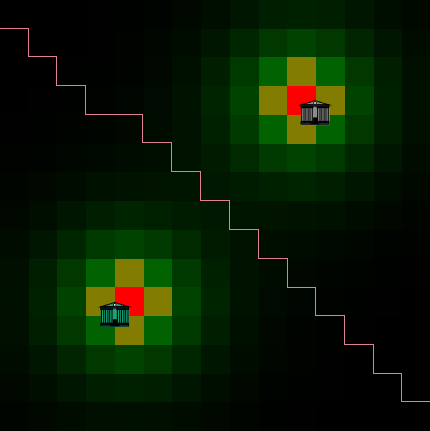
\includegraphics[width=0.49\linewidth]{Figures/Lutecia/ex_setup.png}
	%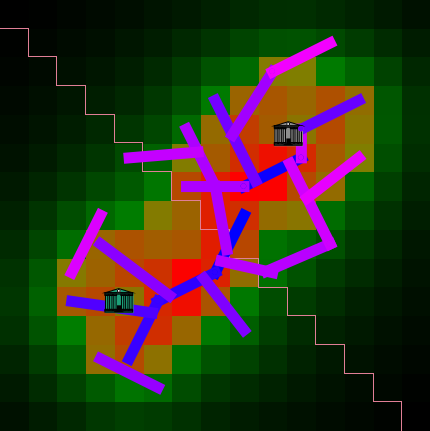
\includegraphics[width=0.49\linewidth]{Figures/Lutecia/ex_reg_infra50.png}
	%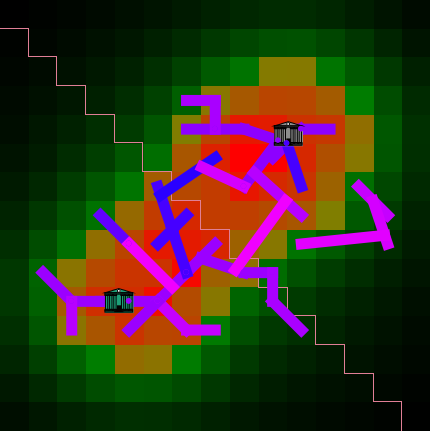
\includegraphics[width=0.49\linewidth]{Figures/Lutecia/ex_maxcollabcost_infra50.png}
	%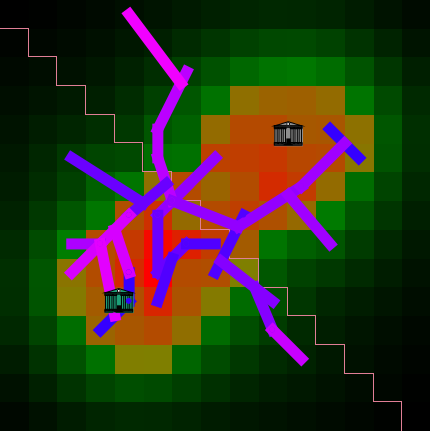
\includegraphics[width=0.49\linewidth]{Figures/Lutecia/ex_mincollabcost_infra50.png}
	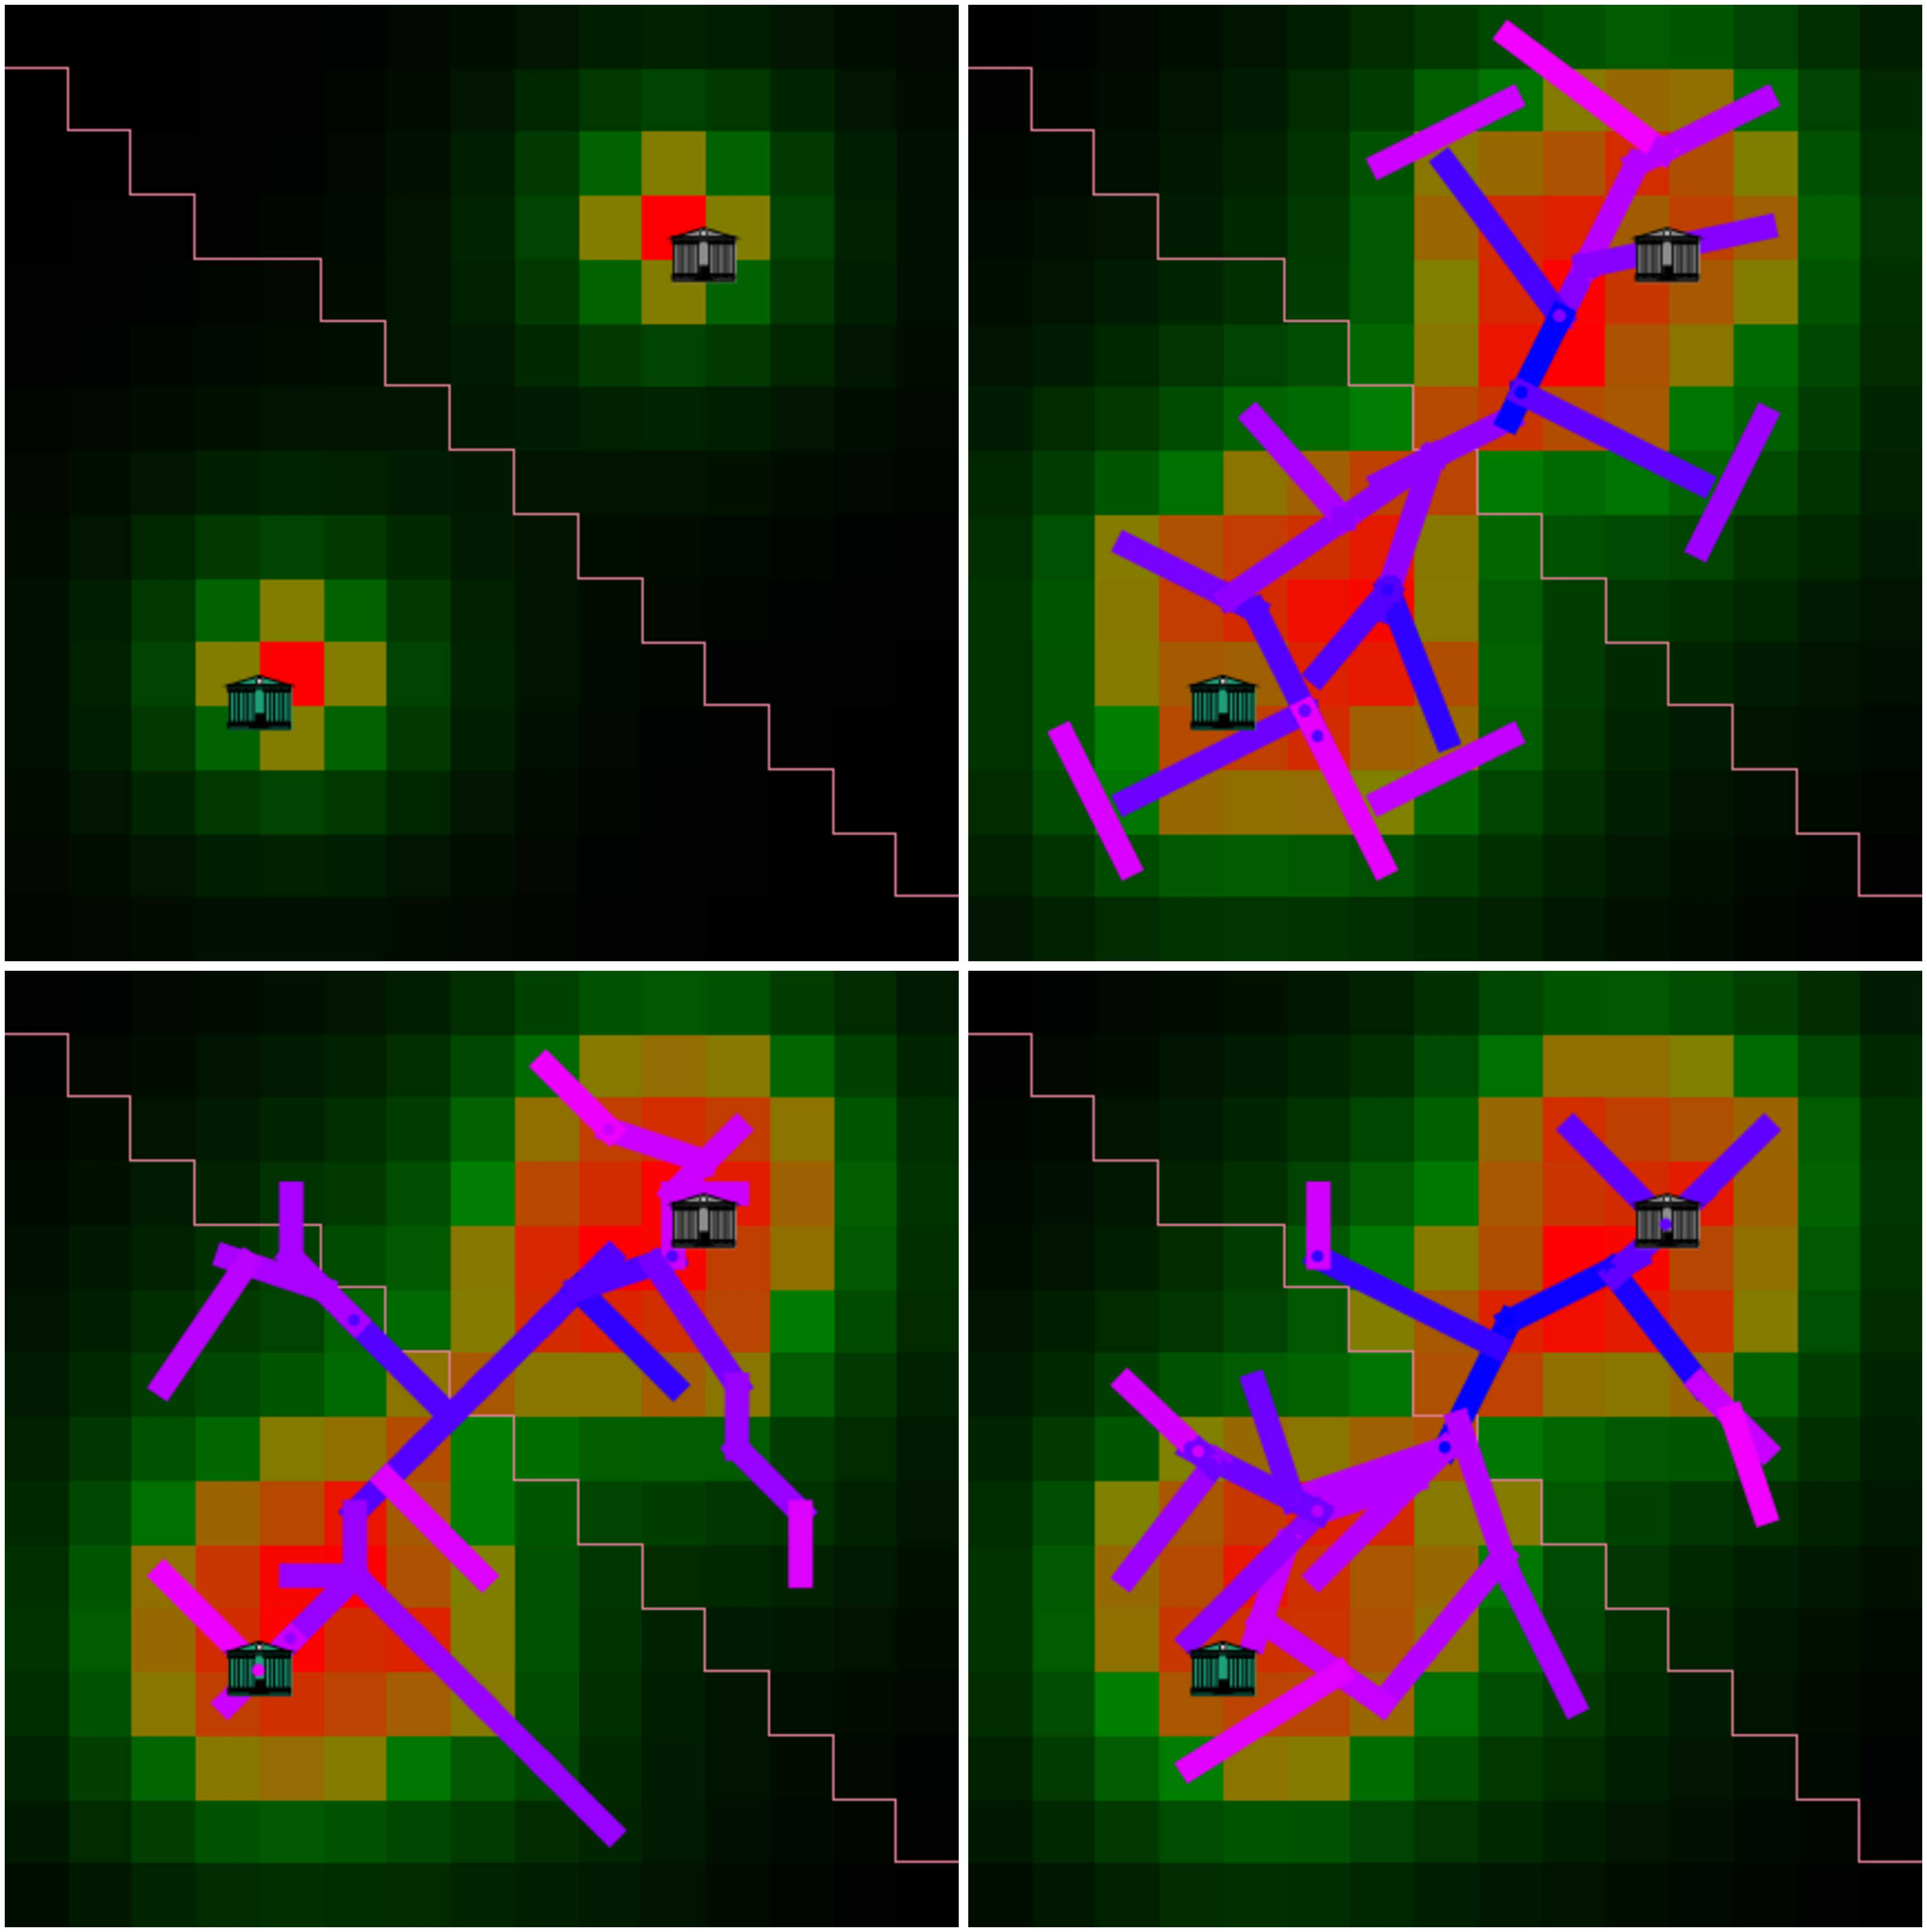
\includegraphics[width=\linewidth]{Figures/Final/7-3-3-fig-lutecia-governance.jpg}
	\caption[Network topologies obtained for different levels of governance][Formes de réseau obtenues pour différents niveaux de gouvernance]{\textbf{Network topologies obtained for different levels of governance.}\label{fig:lutecia:governance}}{\textbf{Formes de réseau obtenues pour différents niveaux de gouvernance.} Le modèle est initialisé sur une configuration synthétique symétrique à deux centres (\textit{Haut gauche}). Les paramètres pour l'évolution de l'usage du sol sont $\gamma_A = \gamma_E = 0.8 ; \beta = 2 ; \lambda = 0.001 ; \alpha = 0.16$, et pour l'évolution du réseau $l_r = 2$ et un jeu à choix discrets. L'évolution est stoppée à stock constant $S = 50$ et l'exploration heuristique faite pour $N_e = 200$. (\textit{Haut droite}) Niveau de décision régional ($\xi = 1$) ; (\textit{Bas gauche}) Niveau local ($\xi = 0$) et bas niveau de collaboration, obtenu avec un fort coût de coopération $J=0.005$ ; (\textit{Bas droite}) Niveau local et haut niveau de collaboration, avec $J=0$.\label{fig:lutecia:governance}}
\end{figure}
%%%%%%%%%%%%



\paragraph{Co-evolution}{Co-évolution}

Dans une dernière expérience stylisée, nous proposons d'étudier plus directement l'effet de la co-évolution, notamment sur les variables d'usage du sol.




%%%%%%%%%%%%
\begin{figure}
	%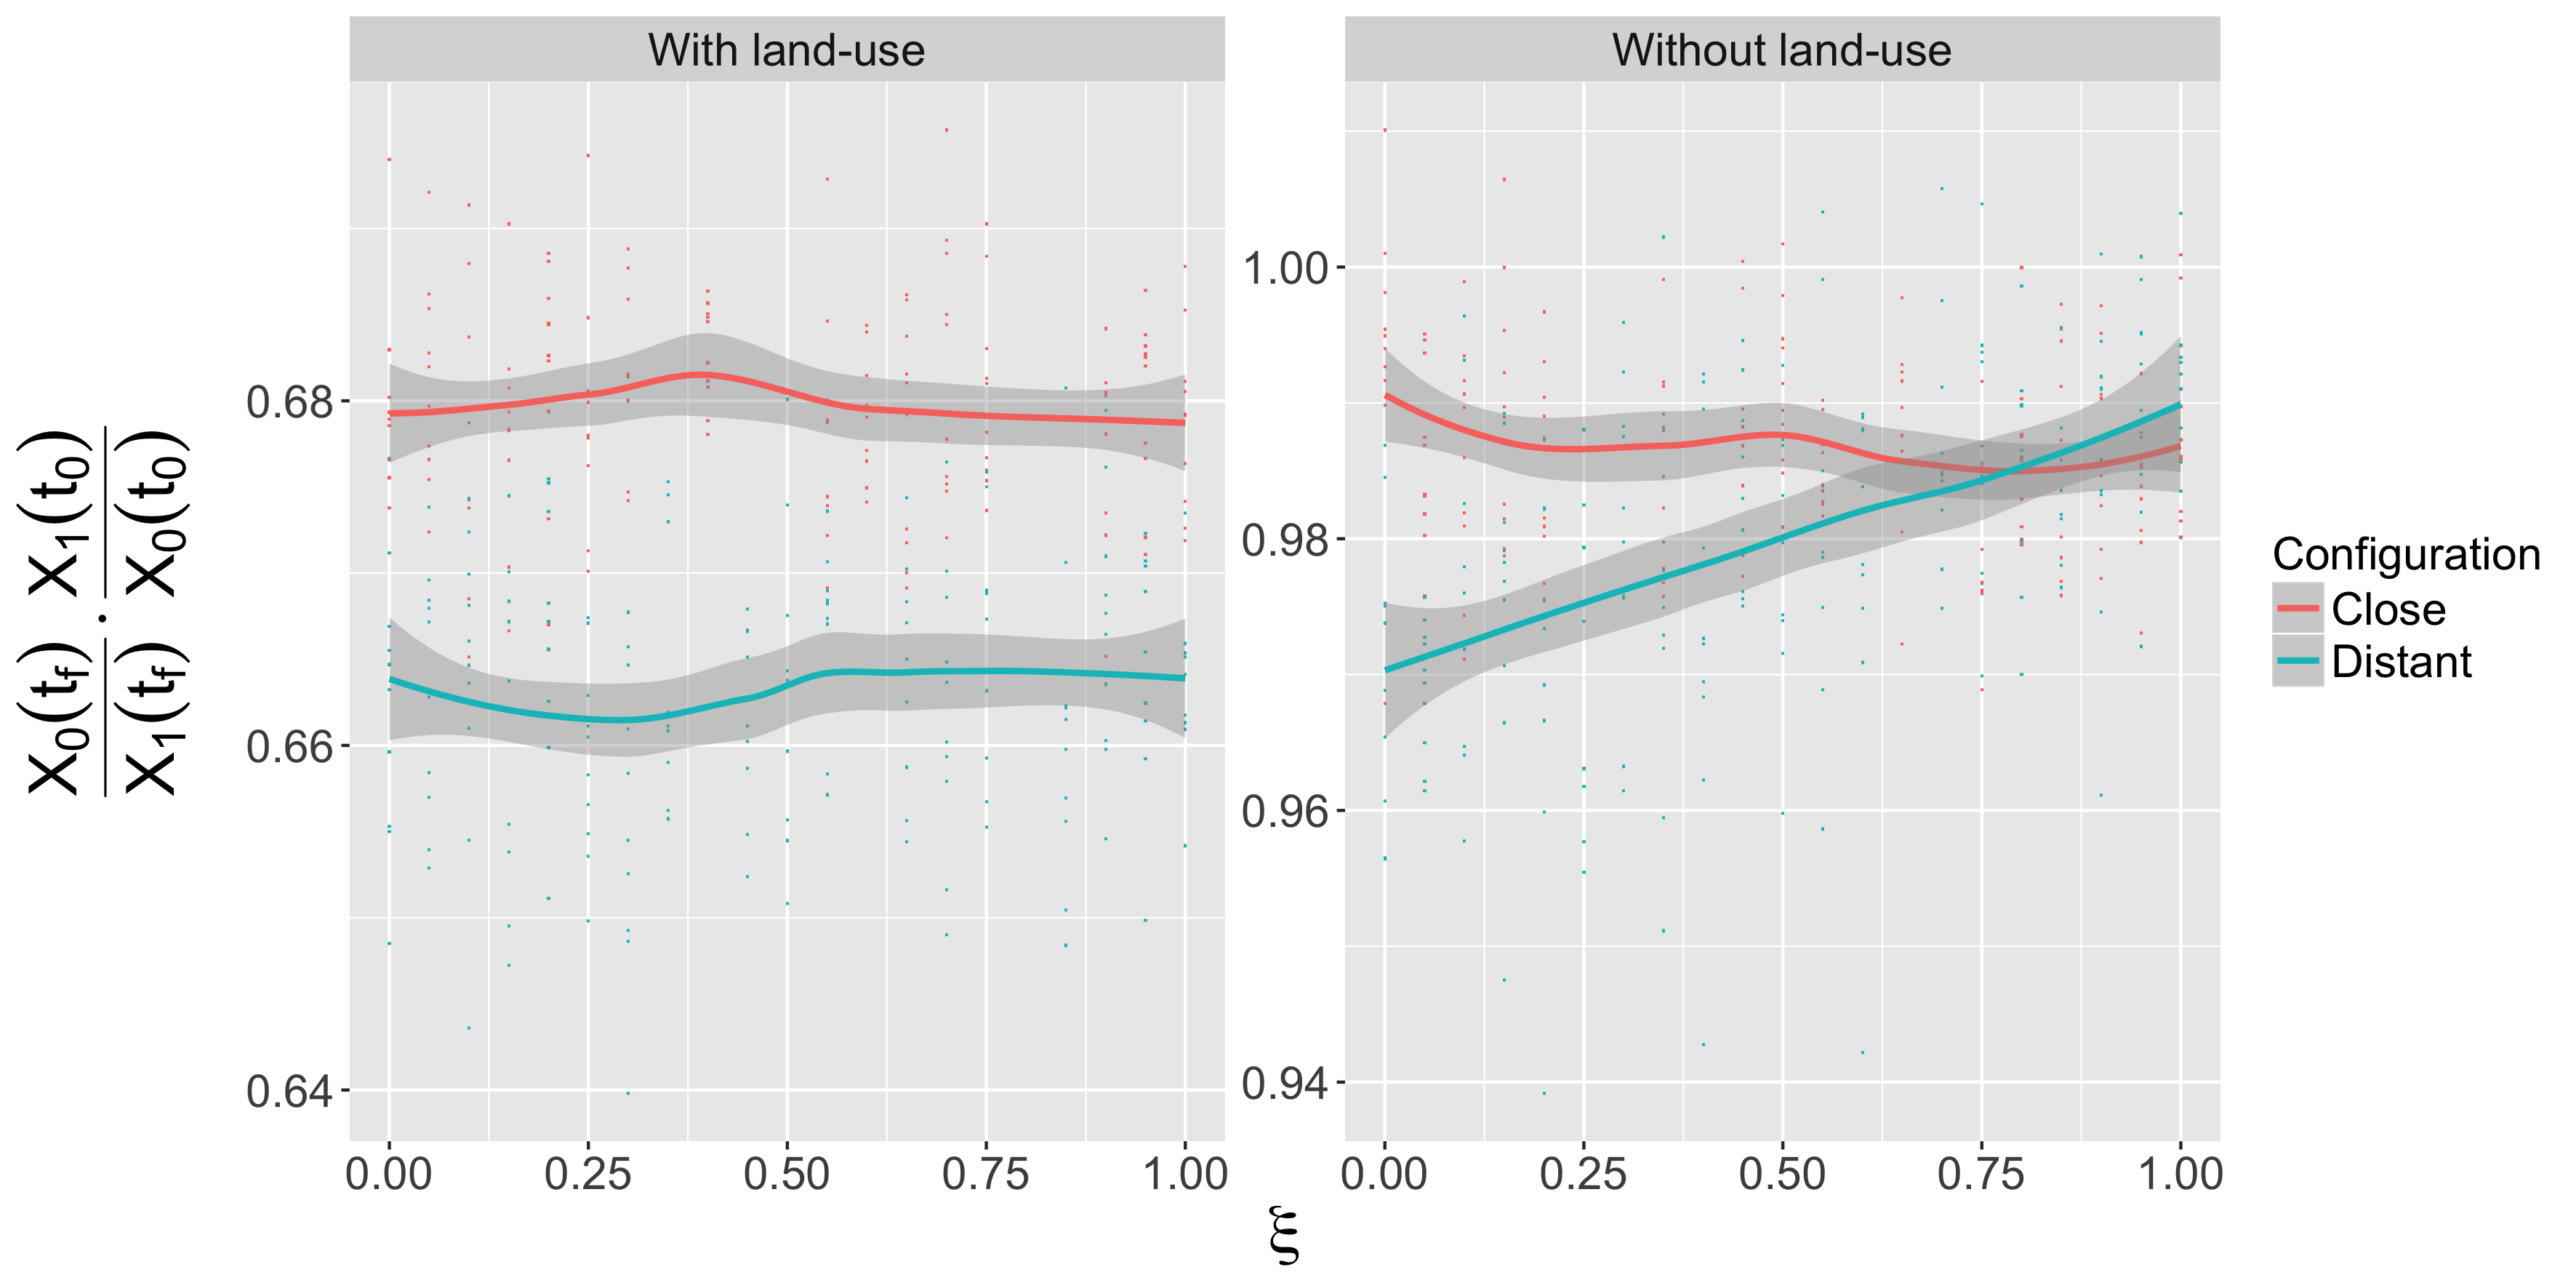
\includegraphics[width=\linewidth]{Figures/Lutecia/accessbalance.png}\\
    %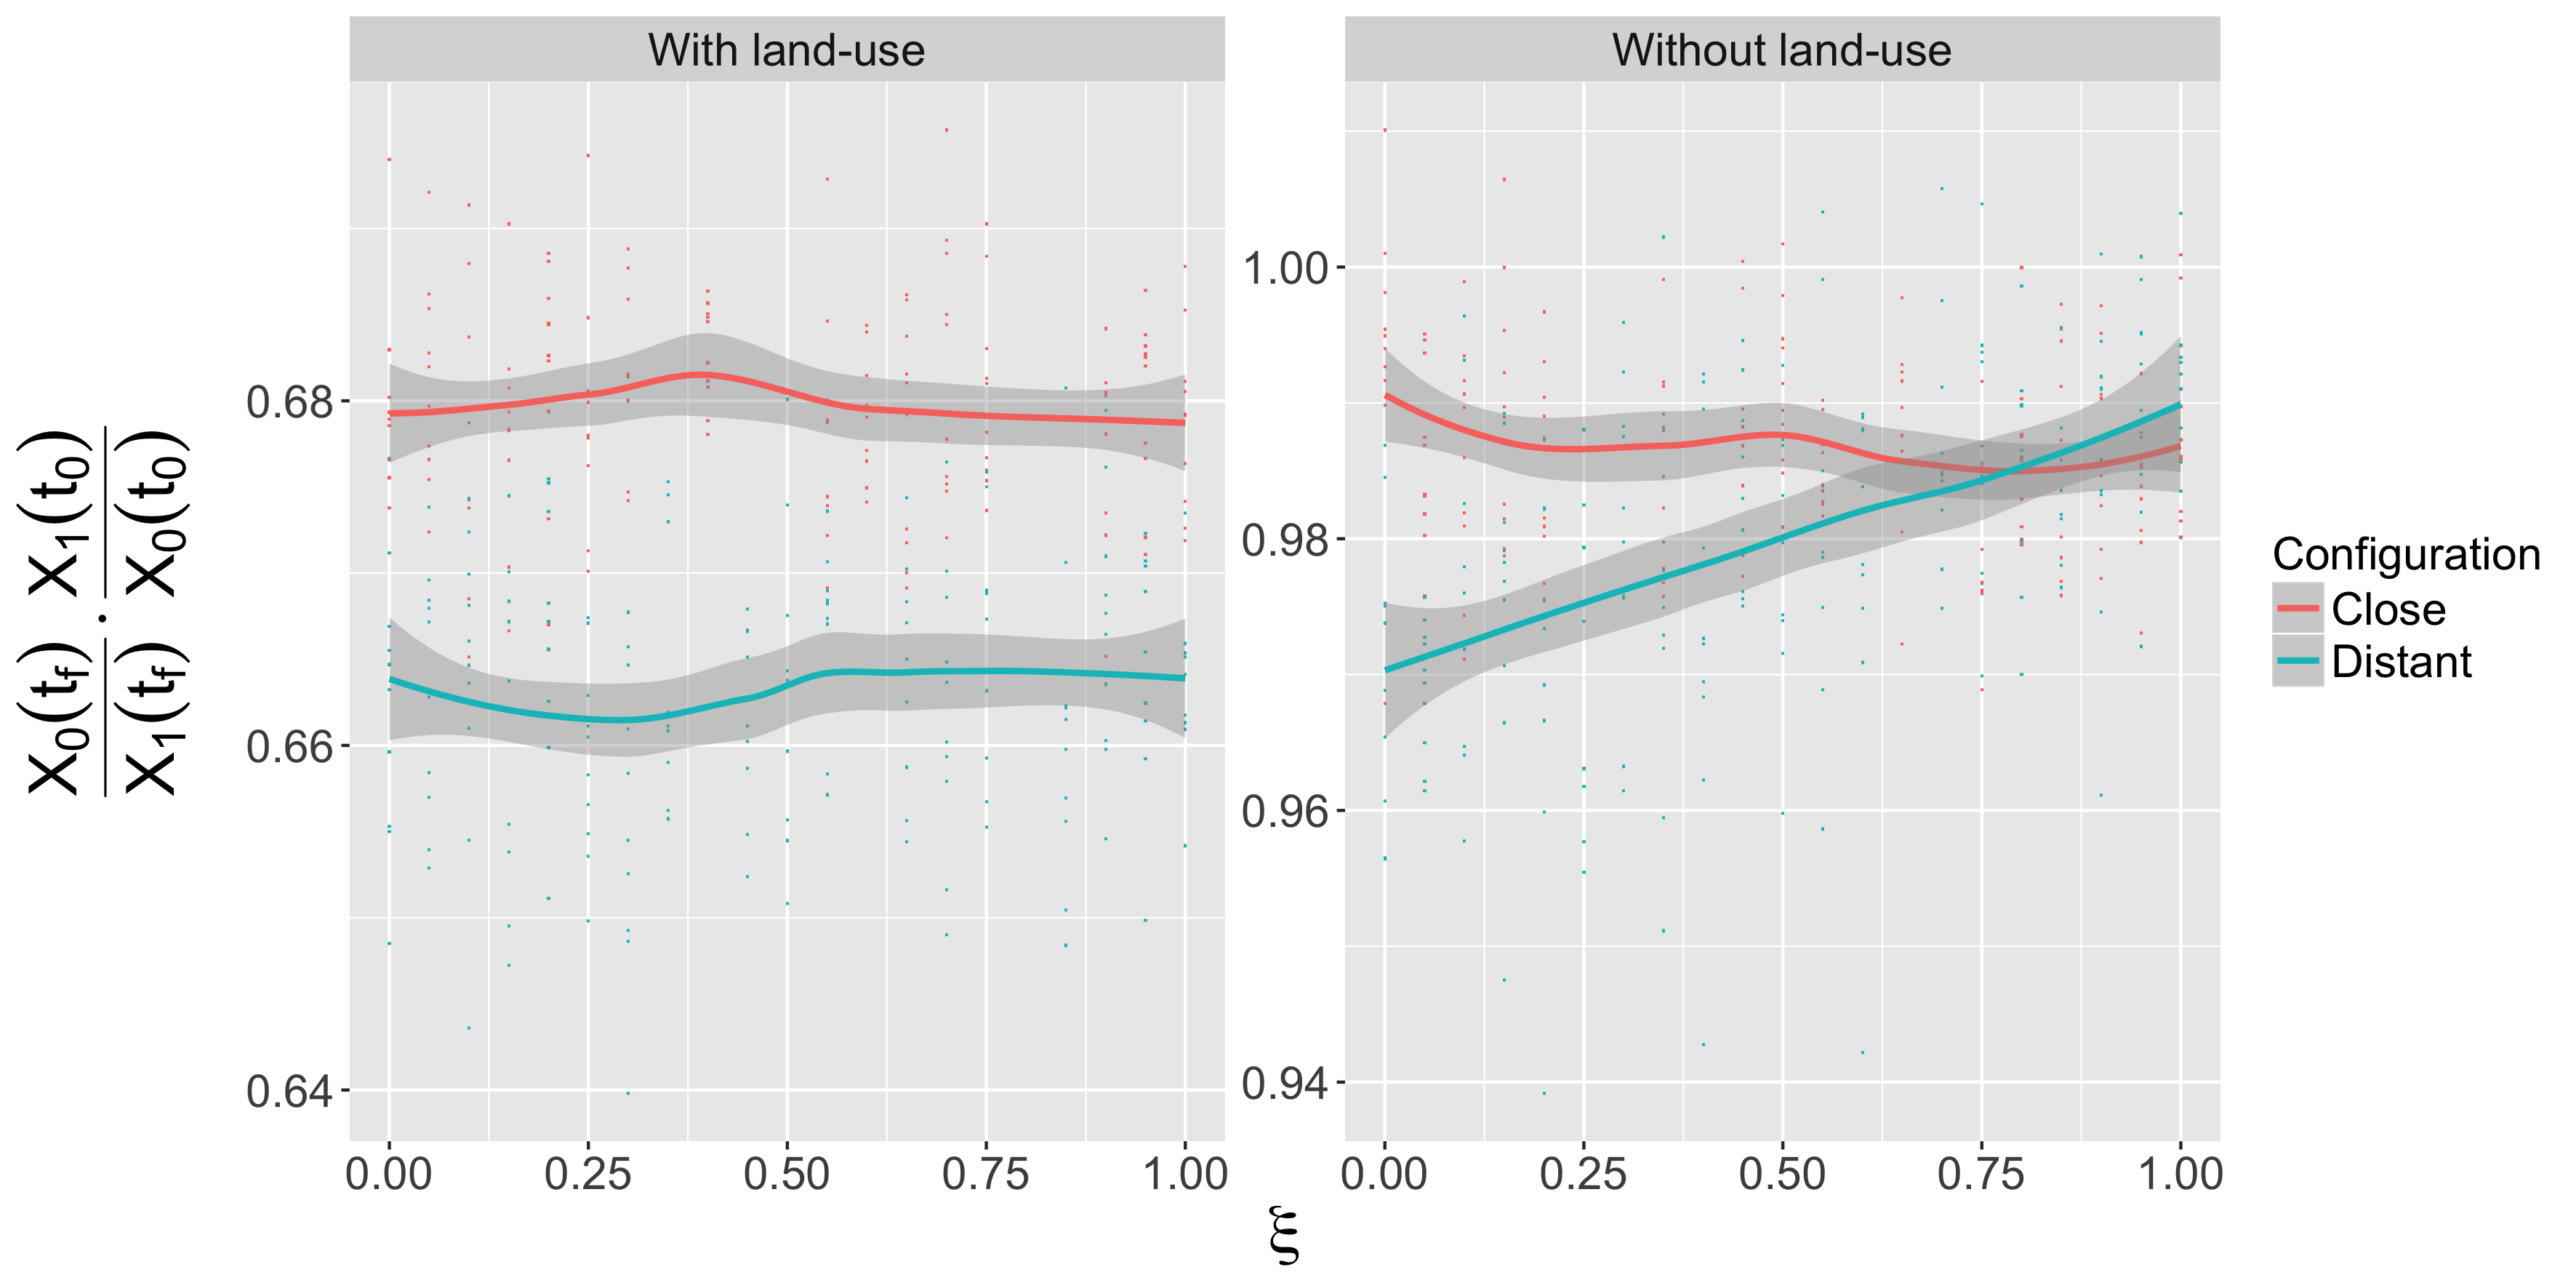
\includegraphics[width=\linewidth]{Figures/Lutecia/accesstot.png}
	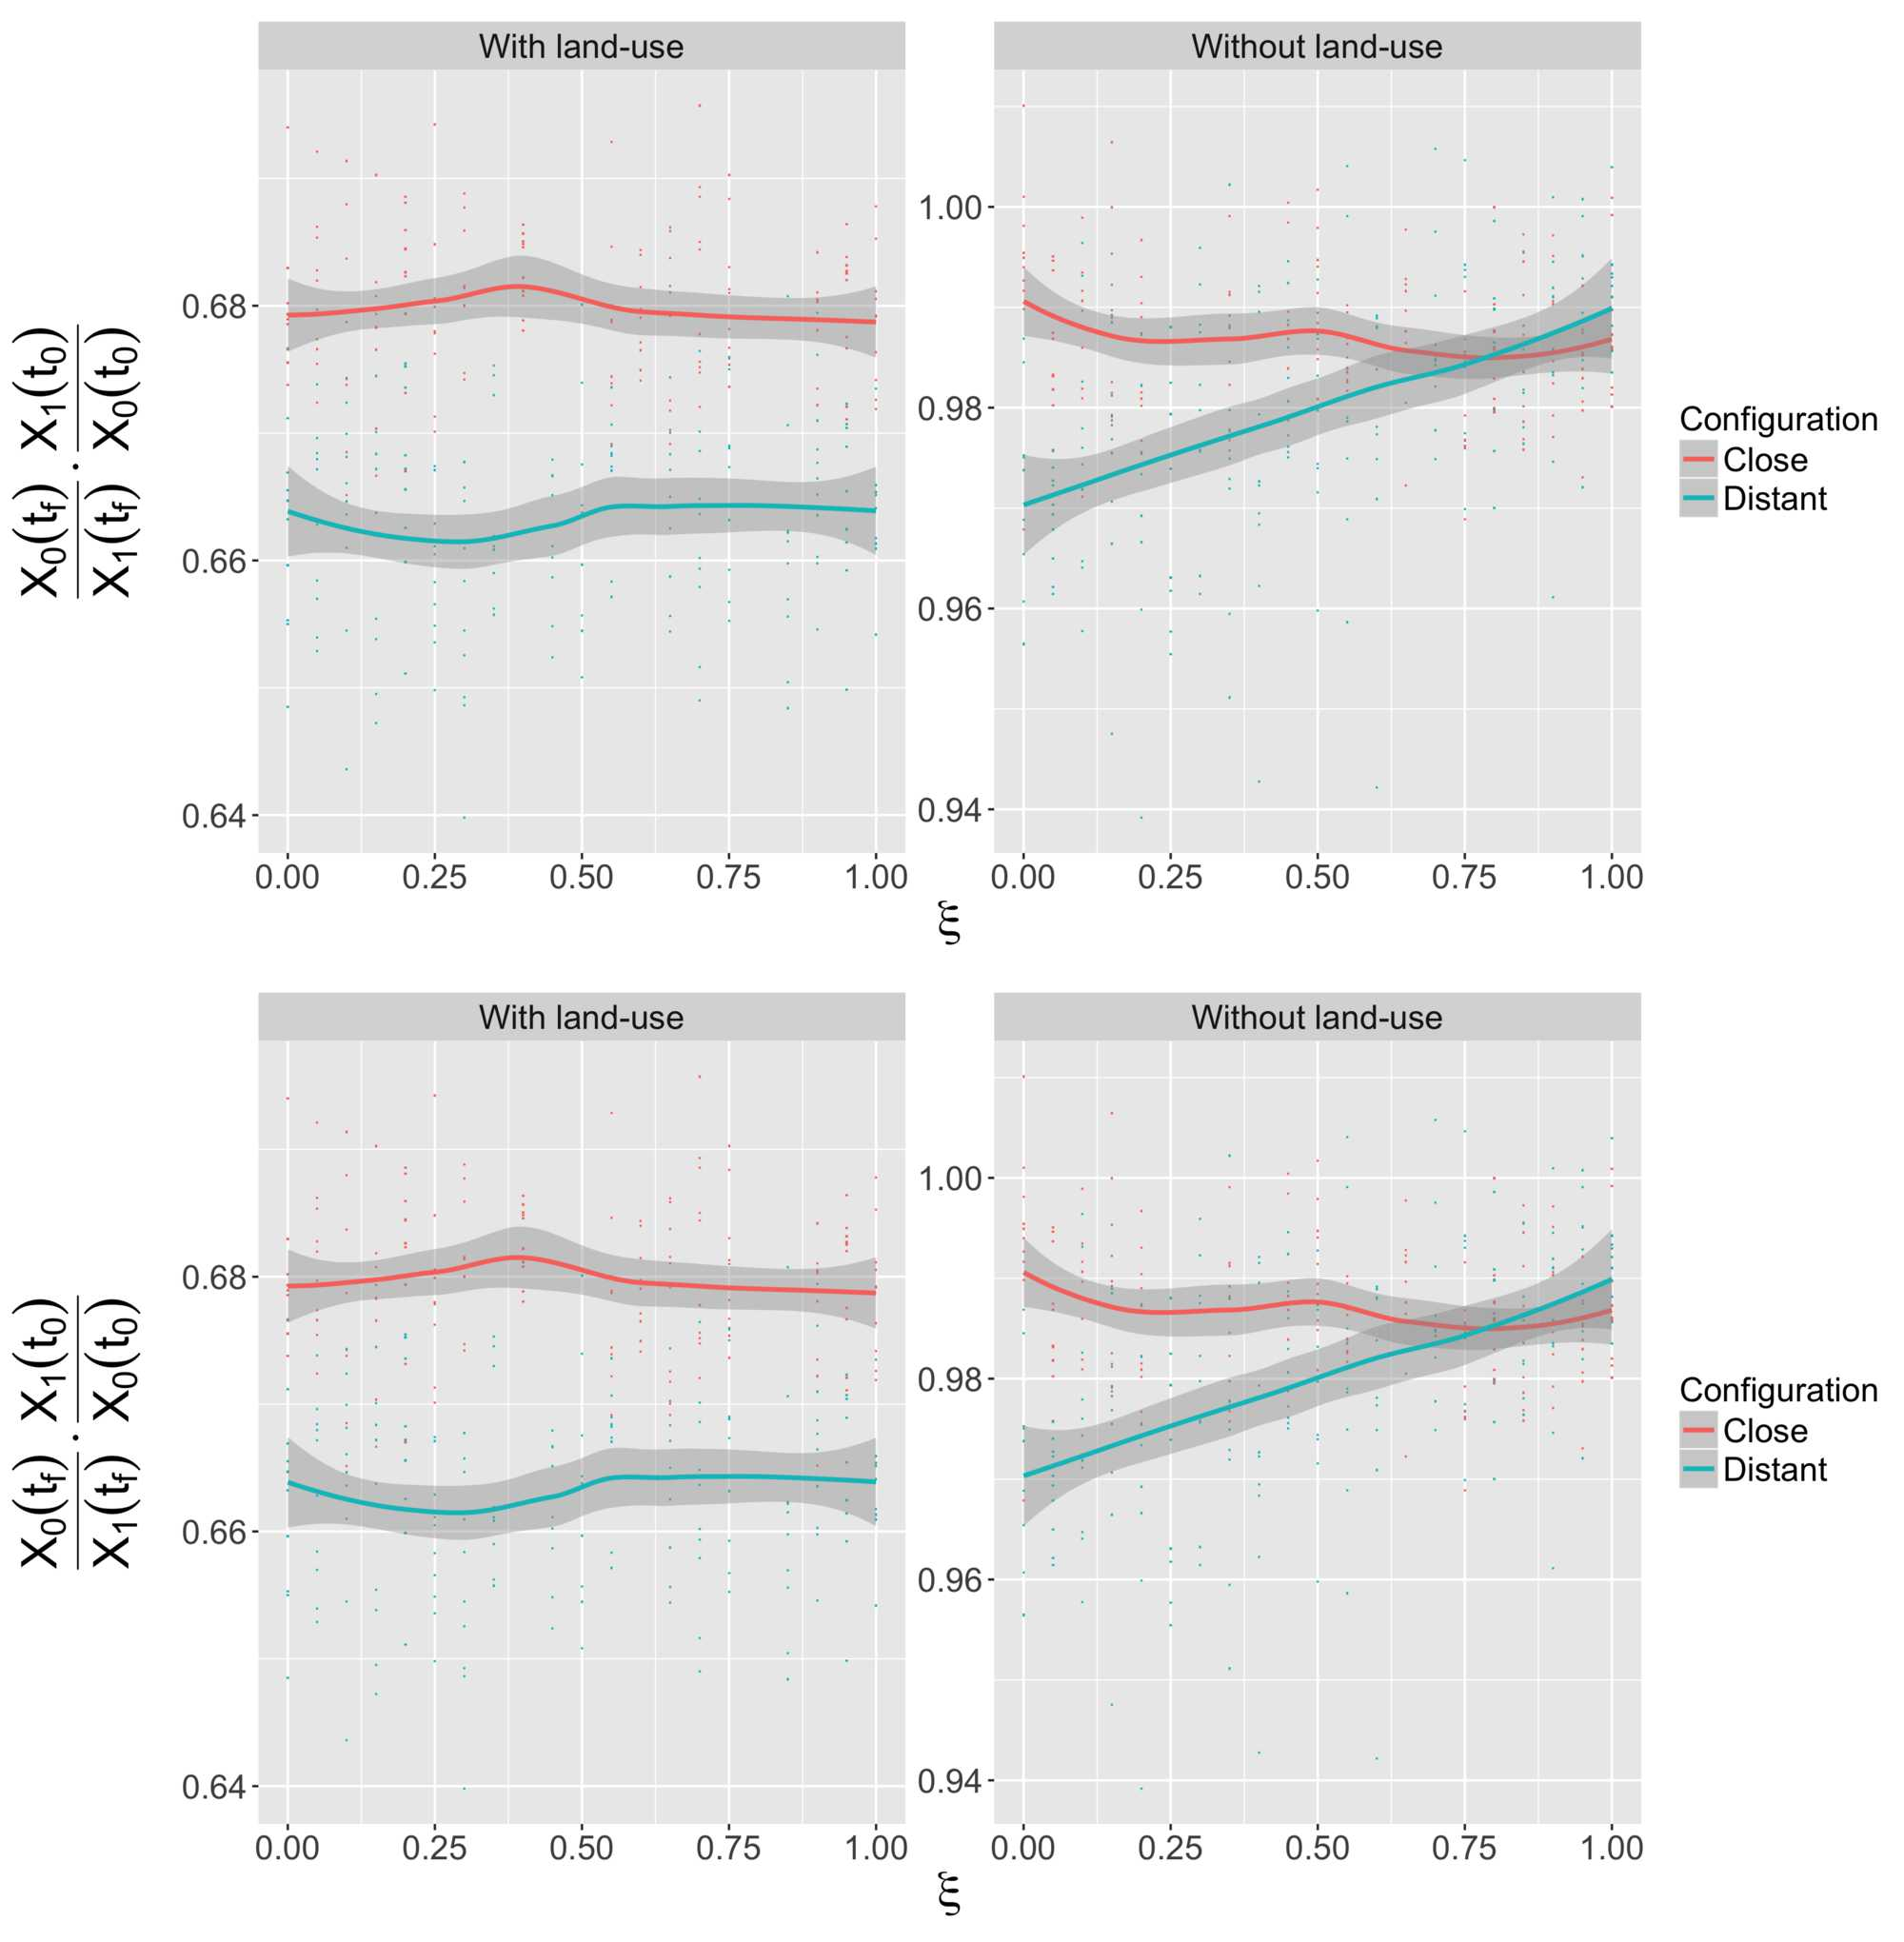
\includegraphics[width=\linewidth]{Figures/Final/7-3-3-fig-lutecia-coevol.jpg}
	\caption[Impact of co-evolution on accessibility in the Lutecia model.][Impact de la co-évolution sur l'accessibilité dans le modèle Lutecia]{\textbf{Impact of co-evolution on accessibility in the Lutecia model.}\label{fig:lutecia:coevol}}{\textbf{Impact de la co-évolution sur l'accessibilité dans le modèle Lutecia.}\label{fig:lutecia:coevol}}
\end{figure}
%%%%%%%%%%%%





%%%%%%%%%%%%%%%%%%%%
\subsection{Application to Pearl River Delta}{Application au Delta de la Rivière des Perles}


\bpar{
It was suggested by \cite{liao2017ouverture} that a sort of multi-level governance recently emerged in China, in the context of economic activities. We try with our model to test the relevance of this paradigm regarding the urban structure of the MCR.
}{
Il a été suggéré par \cite{liao2017ouverture} qu'une forme de gouvernance multi-niveau a récemment émergé en Chine, dans le contexte des activités économiques. Nous tentons par notre modèle de tester la pertinence de ce paradigme au regard de la structure urbaine de la MCR.
}






%
%
\subsubsection{Model setup}{Initialisation du modèle}

\bpar{
We work on a simplified raster configuration for population in Pearl River Delta, and on stylized highway networks. We choose to consider road network only since, following \cite{hou2011transport}, it has been the main driver of changes in accessibility patterns compared to railway network which development is only recent.
}{
Nous travaillons sur une configuration raster simplifiée (cellules de 5km) pour la population du Delta de la Rivière des Perles, ainsi que sur le réseau d'autoroute stylisé. Nous considérons le réseau routier uniquement puisque, selon \cite{hou2011transport}, il s'agit du moteur principal des changements dans les motifs d'accessibilité en comparaison au réseau ferré dont le développement accéléré est récent. Les réseaux sont stylisés à partir du plan donné par~\cite{hou2011transport} qui reproduit les documents officiels de la province du Guangdong en 2010. Nous considérons ainsi le réseau autoroutier en 2010 et celui planifié à cette époque. La Fig.~\ref{fig:lutecia:ex-prd} illustre la configuration stylisée pour le Delta de la Rivière des Perles.
}


%
%We show in Fig.~\ref{fig:ex-prd} an illustration of the stylized setup of the model and of its outcome with standard parameter values.


%%%%%%%%%%%%%%%%%%%%
\begin{figure}
%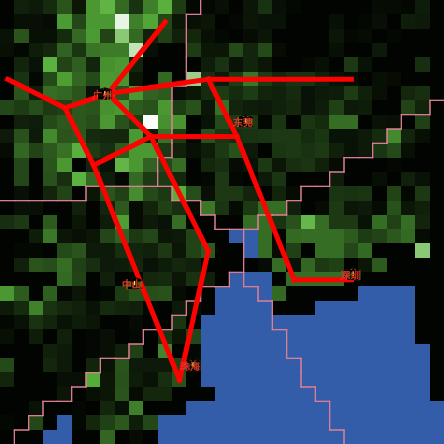
\includegraphics[width=0.49\linewidth]{Figures/Lutecia/exrun_2_tick0}
%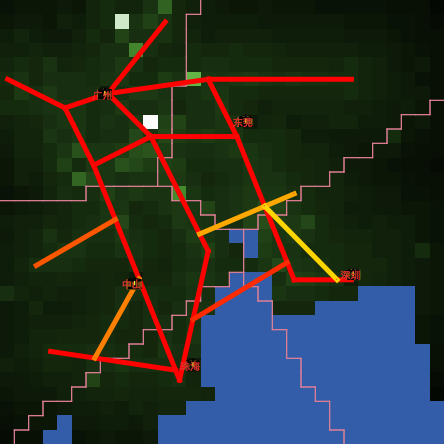
\includegraphics[width=0.49\linewidth]{Figures/Lutecia/exrun_2_tick6}
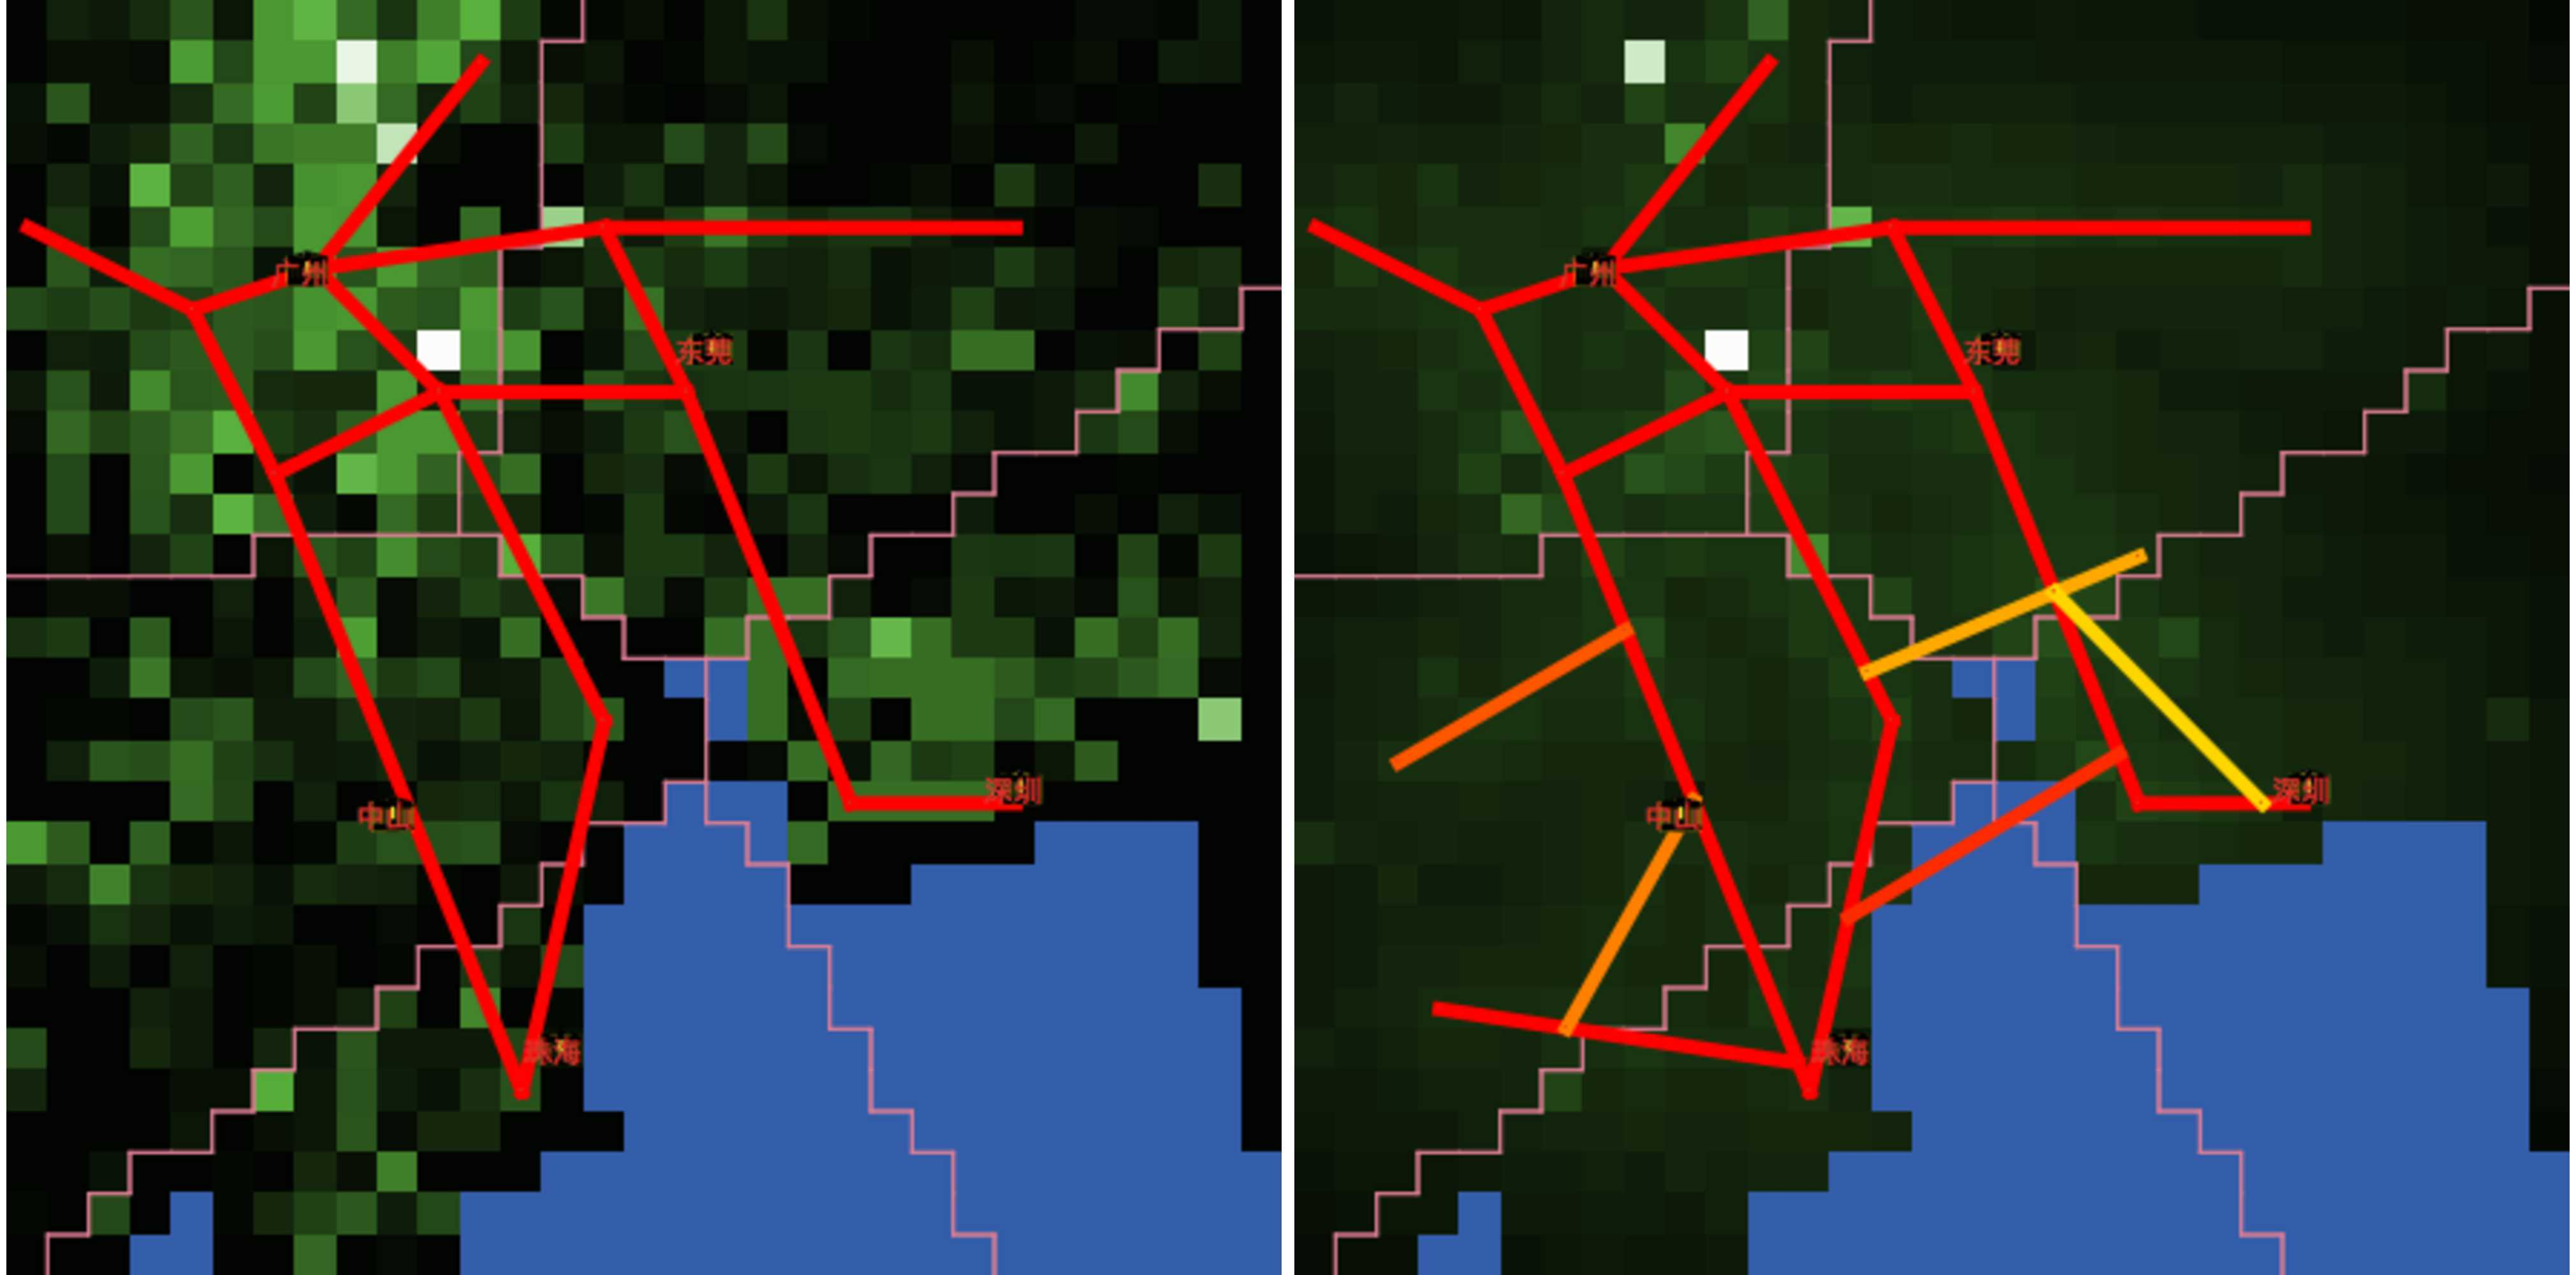
\includegraphics[width=\linewidth]{Figures/Final/7-3-3-fig-lutecia-ex-prd.jpg}
\caption[Application of Lutecia to PRD][Application de Lutecia au Delta de la Rivière des Perles]{\textbf{Example of run on the stylized Pearl River Delta.} (initial configuration and after 6 network iterations)\label{fig:lutecia:ex-prd}}{\textbf{Exemple d'application au Delta de la Rivière des Perles.} (\textit{Gauche}) Initialisation avec le raster de population 2010, agrégé à la résolution 5km, et le réseau autoroutier simplifié ; (\textit{Droite}) Etat après 6 pas de temps ($\alpha = 1$)\label{fig:lutecia:ex-prd}}
\end{figure}
%%%%%%%%%%%%%%%%%%%%





\subsubsection{Calibration procedure}{Procédure de calibration}


\bpar{
To apply such a complex model to a semi-real situation, one must be extremely careful. It is important to choose the adequate processes and level of granularity to reproduce. In particular, our model is not aimed at producing particularly accurate land-use patterns, but uses their approximation as the basis of network growth, which qualitative evolution and the corresponding qualitative patterns in governance processes. We propose therefore to ``calibrate'' on the shape of a given infrastructure, in the sense of determining parameter configurations for which in probability the successive built pieces of infrastructure are the closest to pieces of the target infrastructure. 
}{
Lors de l'application d'un modèle si complexe à une situation semi-réelle, il faut rester vigilant. Il est important de choisir les processus adéquats ainsi que le niveau de granularité à reproduire. En particulier, notre modèle produit des motifs d'usage du sol relativement précis, mais utilise leur approximation comme base de la croissance du réseau, dont l'évolution qualitative permet d'informer sur les processus de gouvernance. Nous proposons pour cela de ``calibrer'' sur la forme d'une infrastructure donnée, au sens de déterminer des configurations de paramètres pour lesquelles en probabilité les morceaux successifs d'infrastructure sont les plus proches d'une infrastructure visée.
}


\bpar{
To calibrate on the network produced by the simulation, it must be compared to a reference network. This is however a difficult problem, as different proximity measures with different significations can be used. Geometrical measures focuses on the spatial proximity of networks. For a network $(E,V)=((e_j),(v_i))$, a node-based distance is given by $\sum_{i \neq i'} d^2 \left(v_i,v_{i'}\right)$. A more accurate measure not biased by intermediate nodes is given by the cumulated area between each pair of edges $\sum_{j \neq j'} A \left(e_j,e_{j'}\right)$ (not a distance in the proper sense) where $A(e,e')$ is the area of the closed polygon formed by joining link extremities.
}{
Pour calibrer sur les réseaux produits par la simulation, il s'agit de comparer à un réseau de référence. C'est un problème difficile, puisque différentes mesures de proximité avec différentes signification peuvent être utilisées. Les mesures géométriques s'intéressent à la proximité spatiale des réseaux. Pour un réseau $(E,V)=((e_j),(v_i))$, une distance basée sur les noeuds est donnée par $\sum_{i \neq i'} d^2 \left(v_i,v_{i'}\right)$. Une mesure plus précise qui n'est pas biaisée par d'éventuels noeuds intermédiaires est donnée par l'aire cumulée entre chaque paire de liens $d_A = \sum_{j \neq j'} A \left(e_j,e_{j'}\right)$ (il ne s'agit pas d'une distance à proprement parler), où $A(e,e')$ est l'aire du polygone fermé constitué en reliant les sommets des liens. Nous considérerons cette dernière pour la calibration.
}




\subsubsection{Calibration}{Calibration}

Les expériences que nous menons sont à usage du sol fixé, le niveau de détail requis pour des données plus anciennes et plus récentes, voir des projections, pour la population et les emplois n'étant pas permis par les données à notre disposition.

Nous faisons varier les paramètres de gouvernance, incluant le type de jeu, avec $l_r = 2$ fixé, et explorons un échantillonnage LHS de 4000 points dans l'espace de ces paramètres, avec 10 répétitions du modèle pour chaque point. Les deux expériences menées correspondent à des configurations cible différentes :
\begin{itemize}
	\item pas de réseau initial et réseau de 2010 comme cible, dans l'esprit d'extrapoler la configuration de gouvernance la plus probable ayant mené à la configuration actuelle ;
	\item réseau 2010 initial, et réseau planifié comme cible : extrapolation de la configuration de gouvernance de la planification.
\end{itemize}

Nous obtenons des résultats qualitativement similaires pour les deux expériences, suggérant qu'il n'y a pas eu de transition de type de gouvernance entre réseau passé et réseau futur. Les résultats sont illustrés en Fig.~\ref{fig:lutecia:calib}. On obtient, à l'étude du graphe de $d_A$ en fonction de $\xi$, que le niveau régional est le plus fidèle pour reproduire la forme du réseau. Par contre, les jeux de choix discrets et de compétition se comporte différemment, et le jeu compétitif est le plus proche de la réalité quand $\xi$ diminue : les relations entre acteurs locaux seraient a priori de nature plus compétitive qu'égoïste. Quand on étudie la variation de la distance en fonction du niveau de collaboration observé, on obtient une forme intéressante en cloche inversée, c'est à dire que les situations les plus probables sont soit celles où il n'y a que de la collaboration, soit celles où il n'y en a pas du tout, mais pas de situations intermédiaires. Enfin, la comparaison des distributions statistiques des distances entre les configurations cibles et les types de jeux montre que la différence entre les jeux n'est considérable que pour le réseau réel mais pas le réseau planifié (conclusion difficile à interpréter).



%%%%%%%%%%%%%%%
\begin{figure}
	%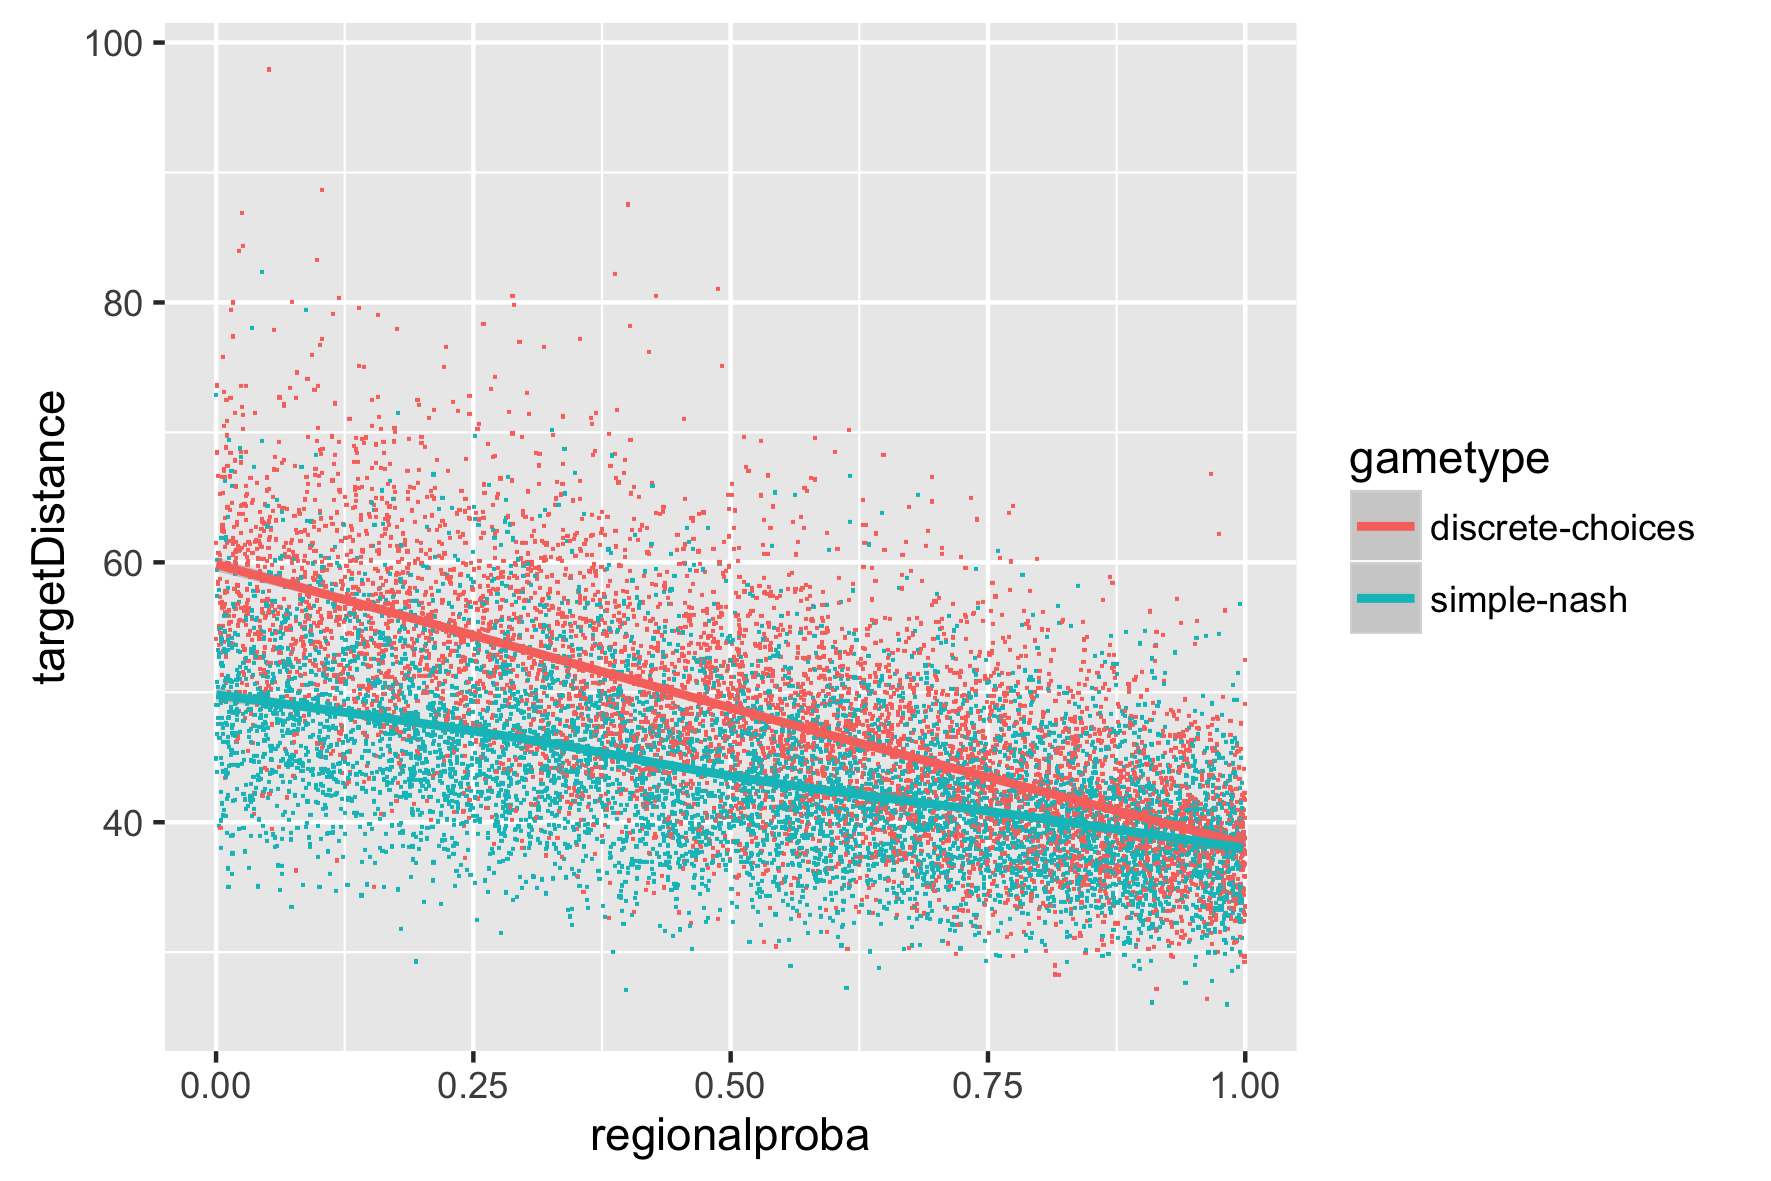
\includegraphics[width=0.49\linewidth]{Figures/Lutecia/regional-distance_colorgametype.png}
	%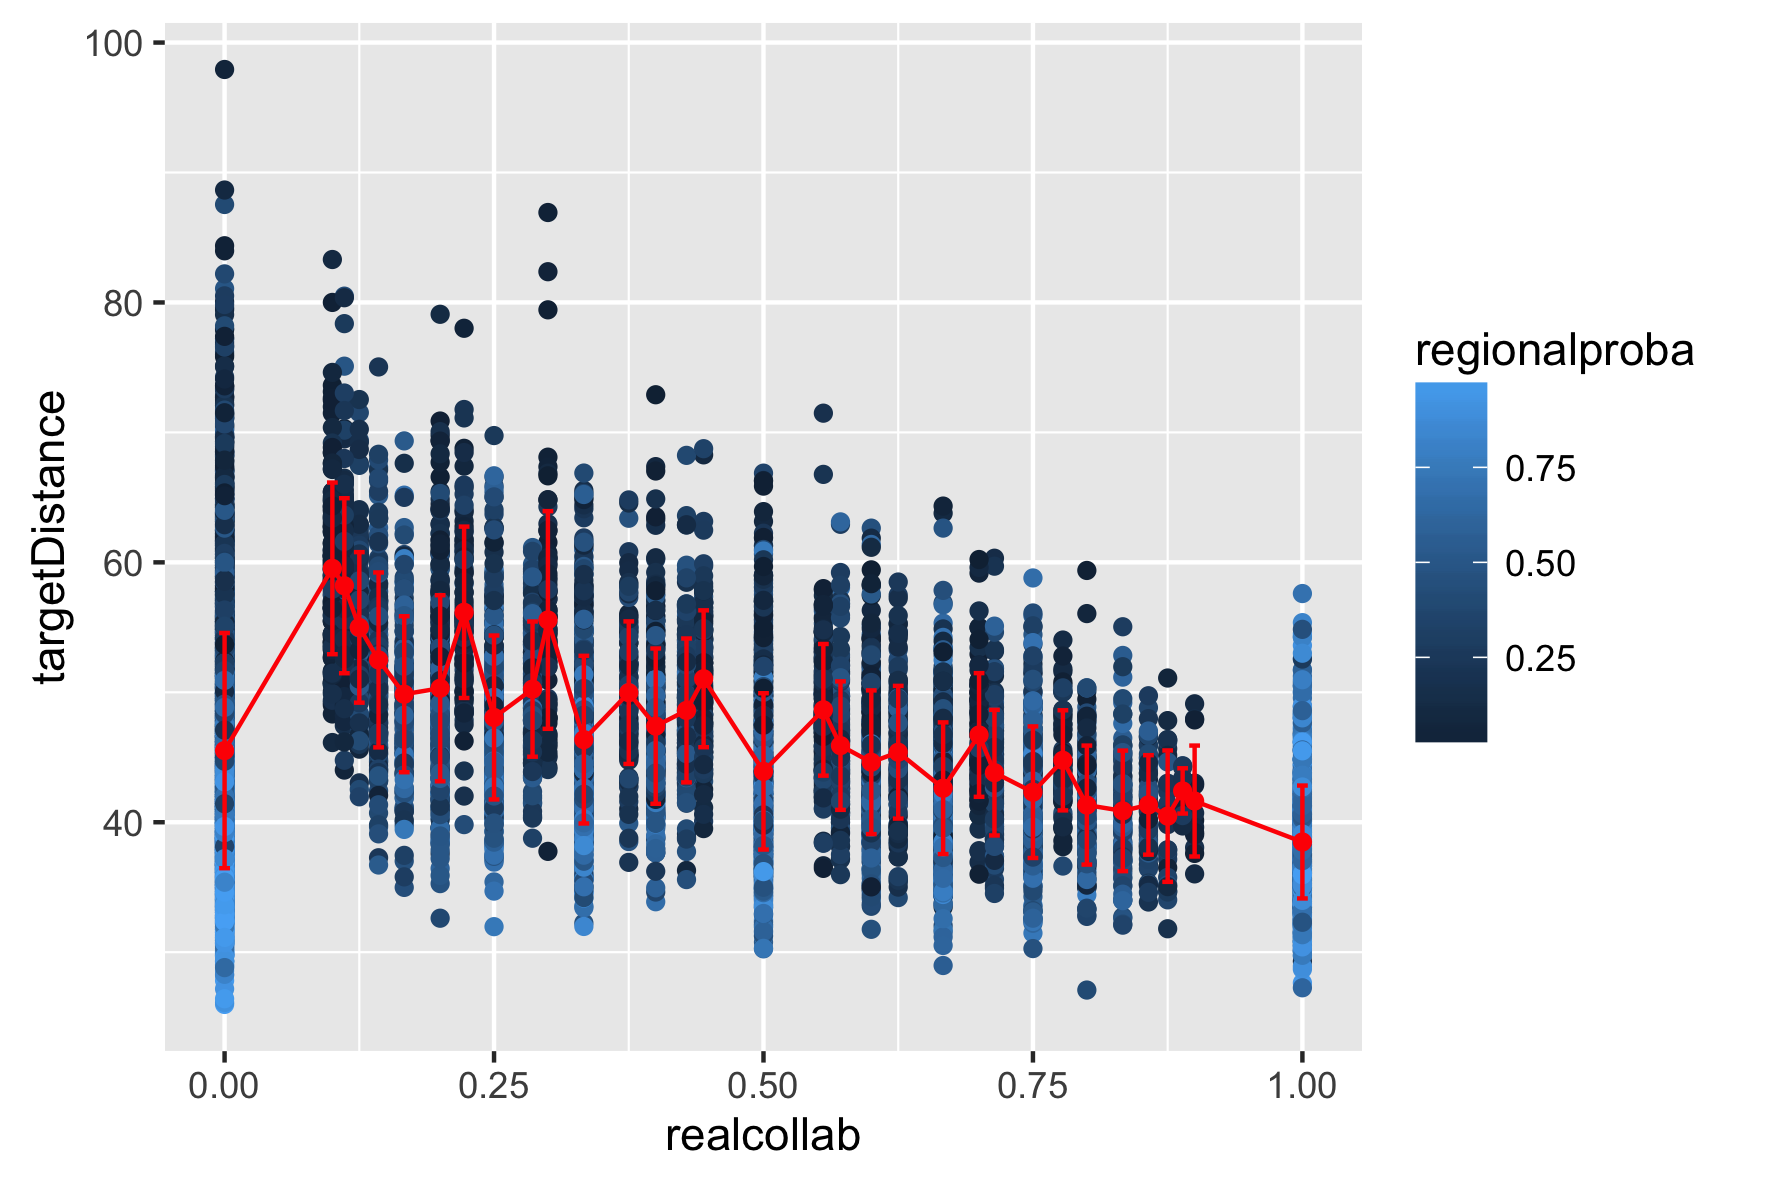
\includegraphics[width=0.49\linewidth]{Figures/Lutecia/collab-distance_colorregional.png}
	%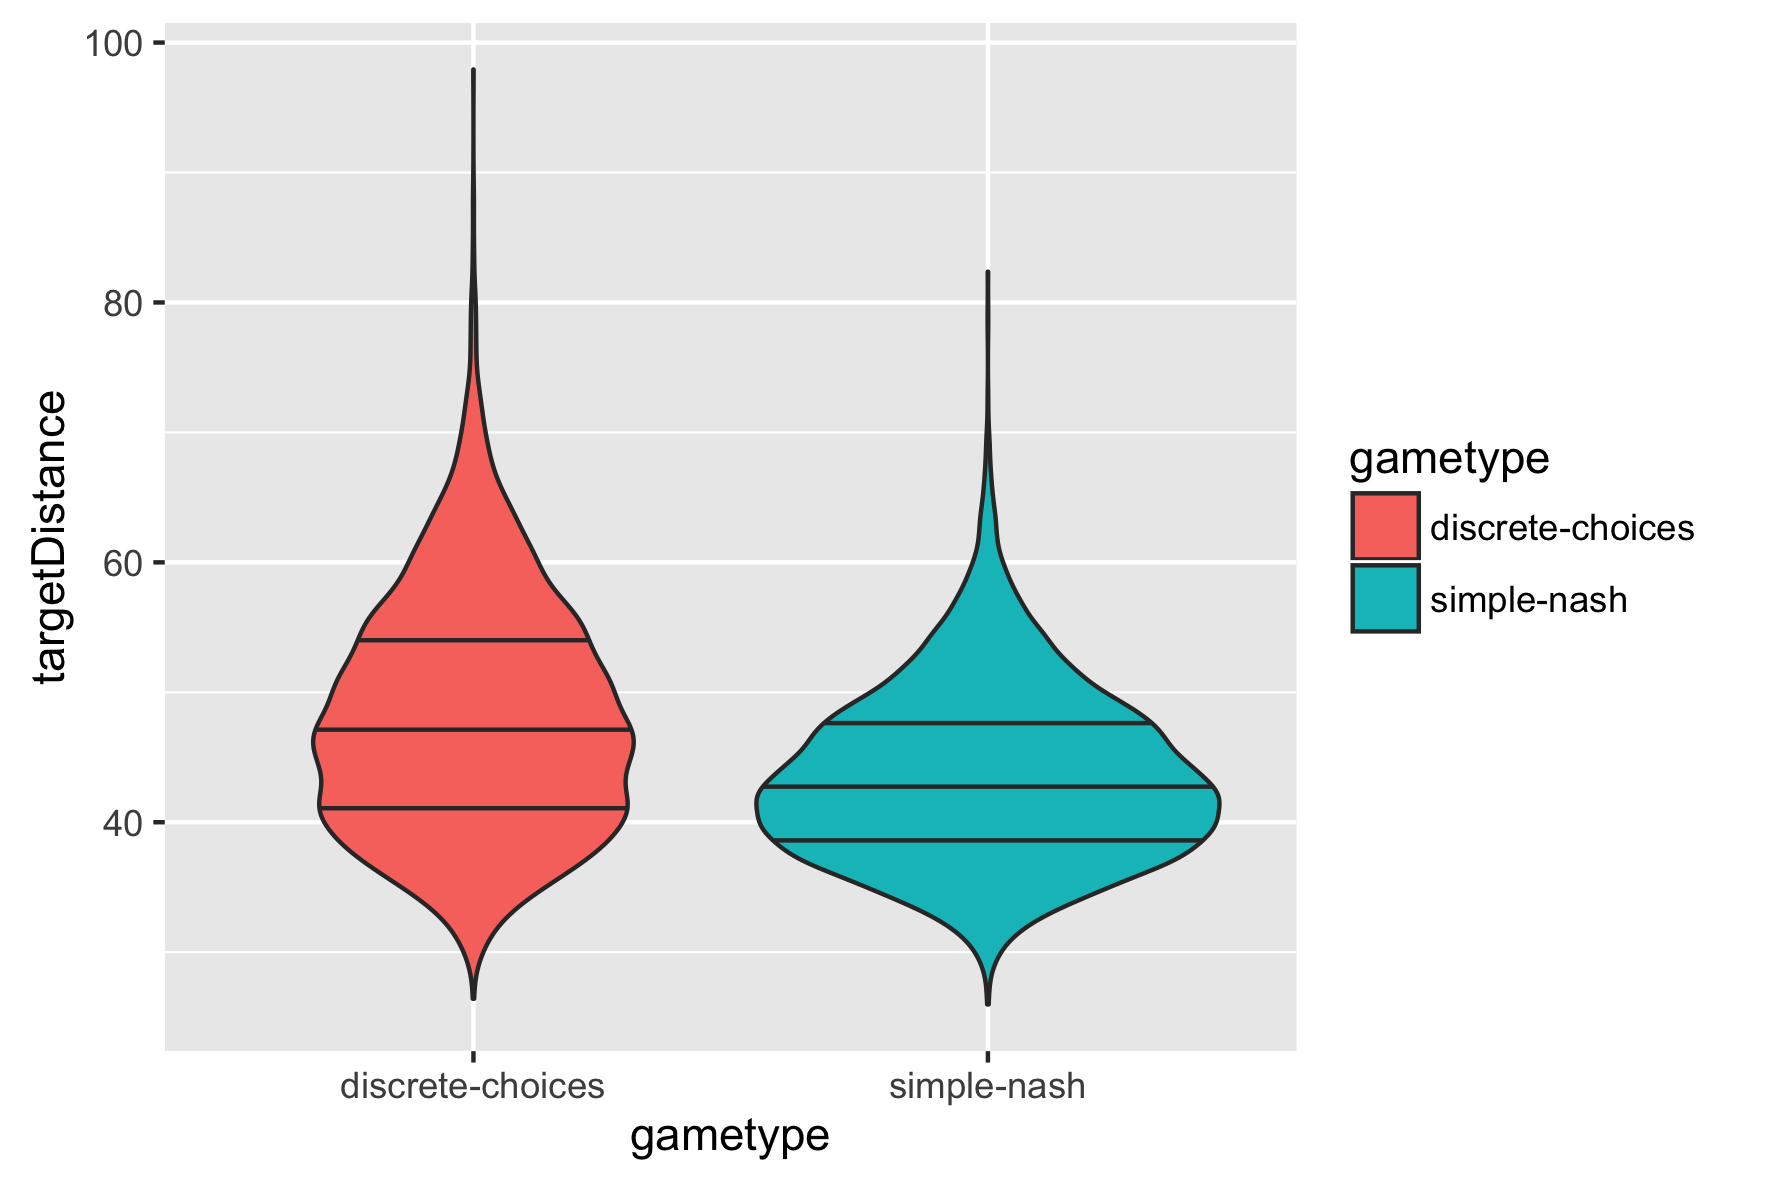
\includegraphics[width=0.49\linewidth]{Figures/Lutecia/distanceviolin_gametype.png}
	%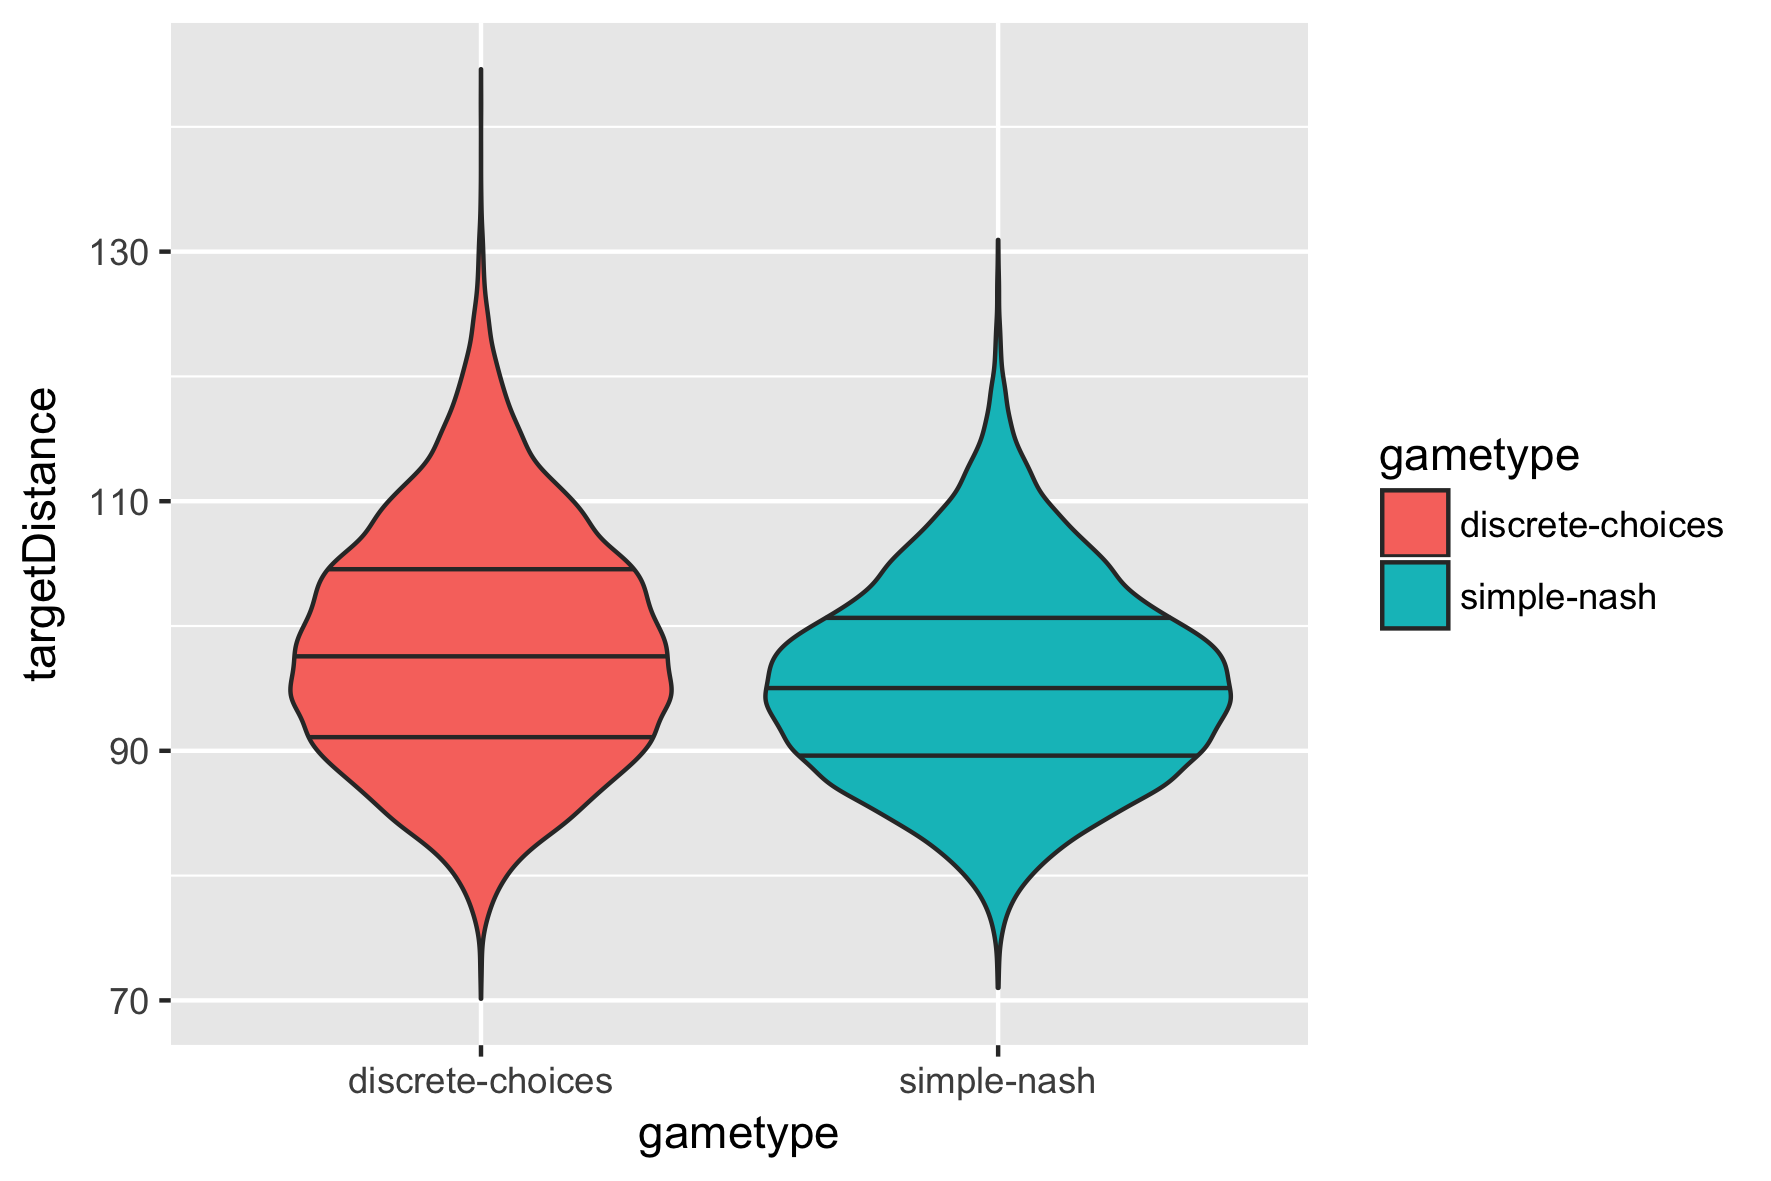
\includegraphics[width=0.49\linewidth]{Figures/Lutecia/distanceviolin_gametype_real.png}
	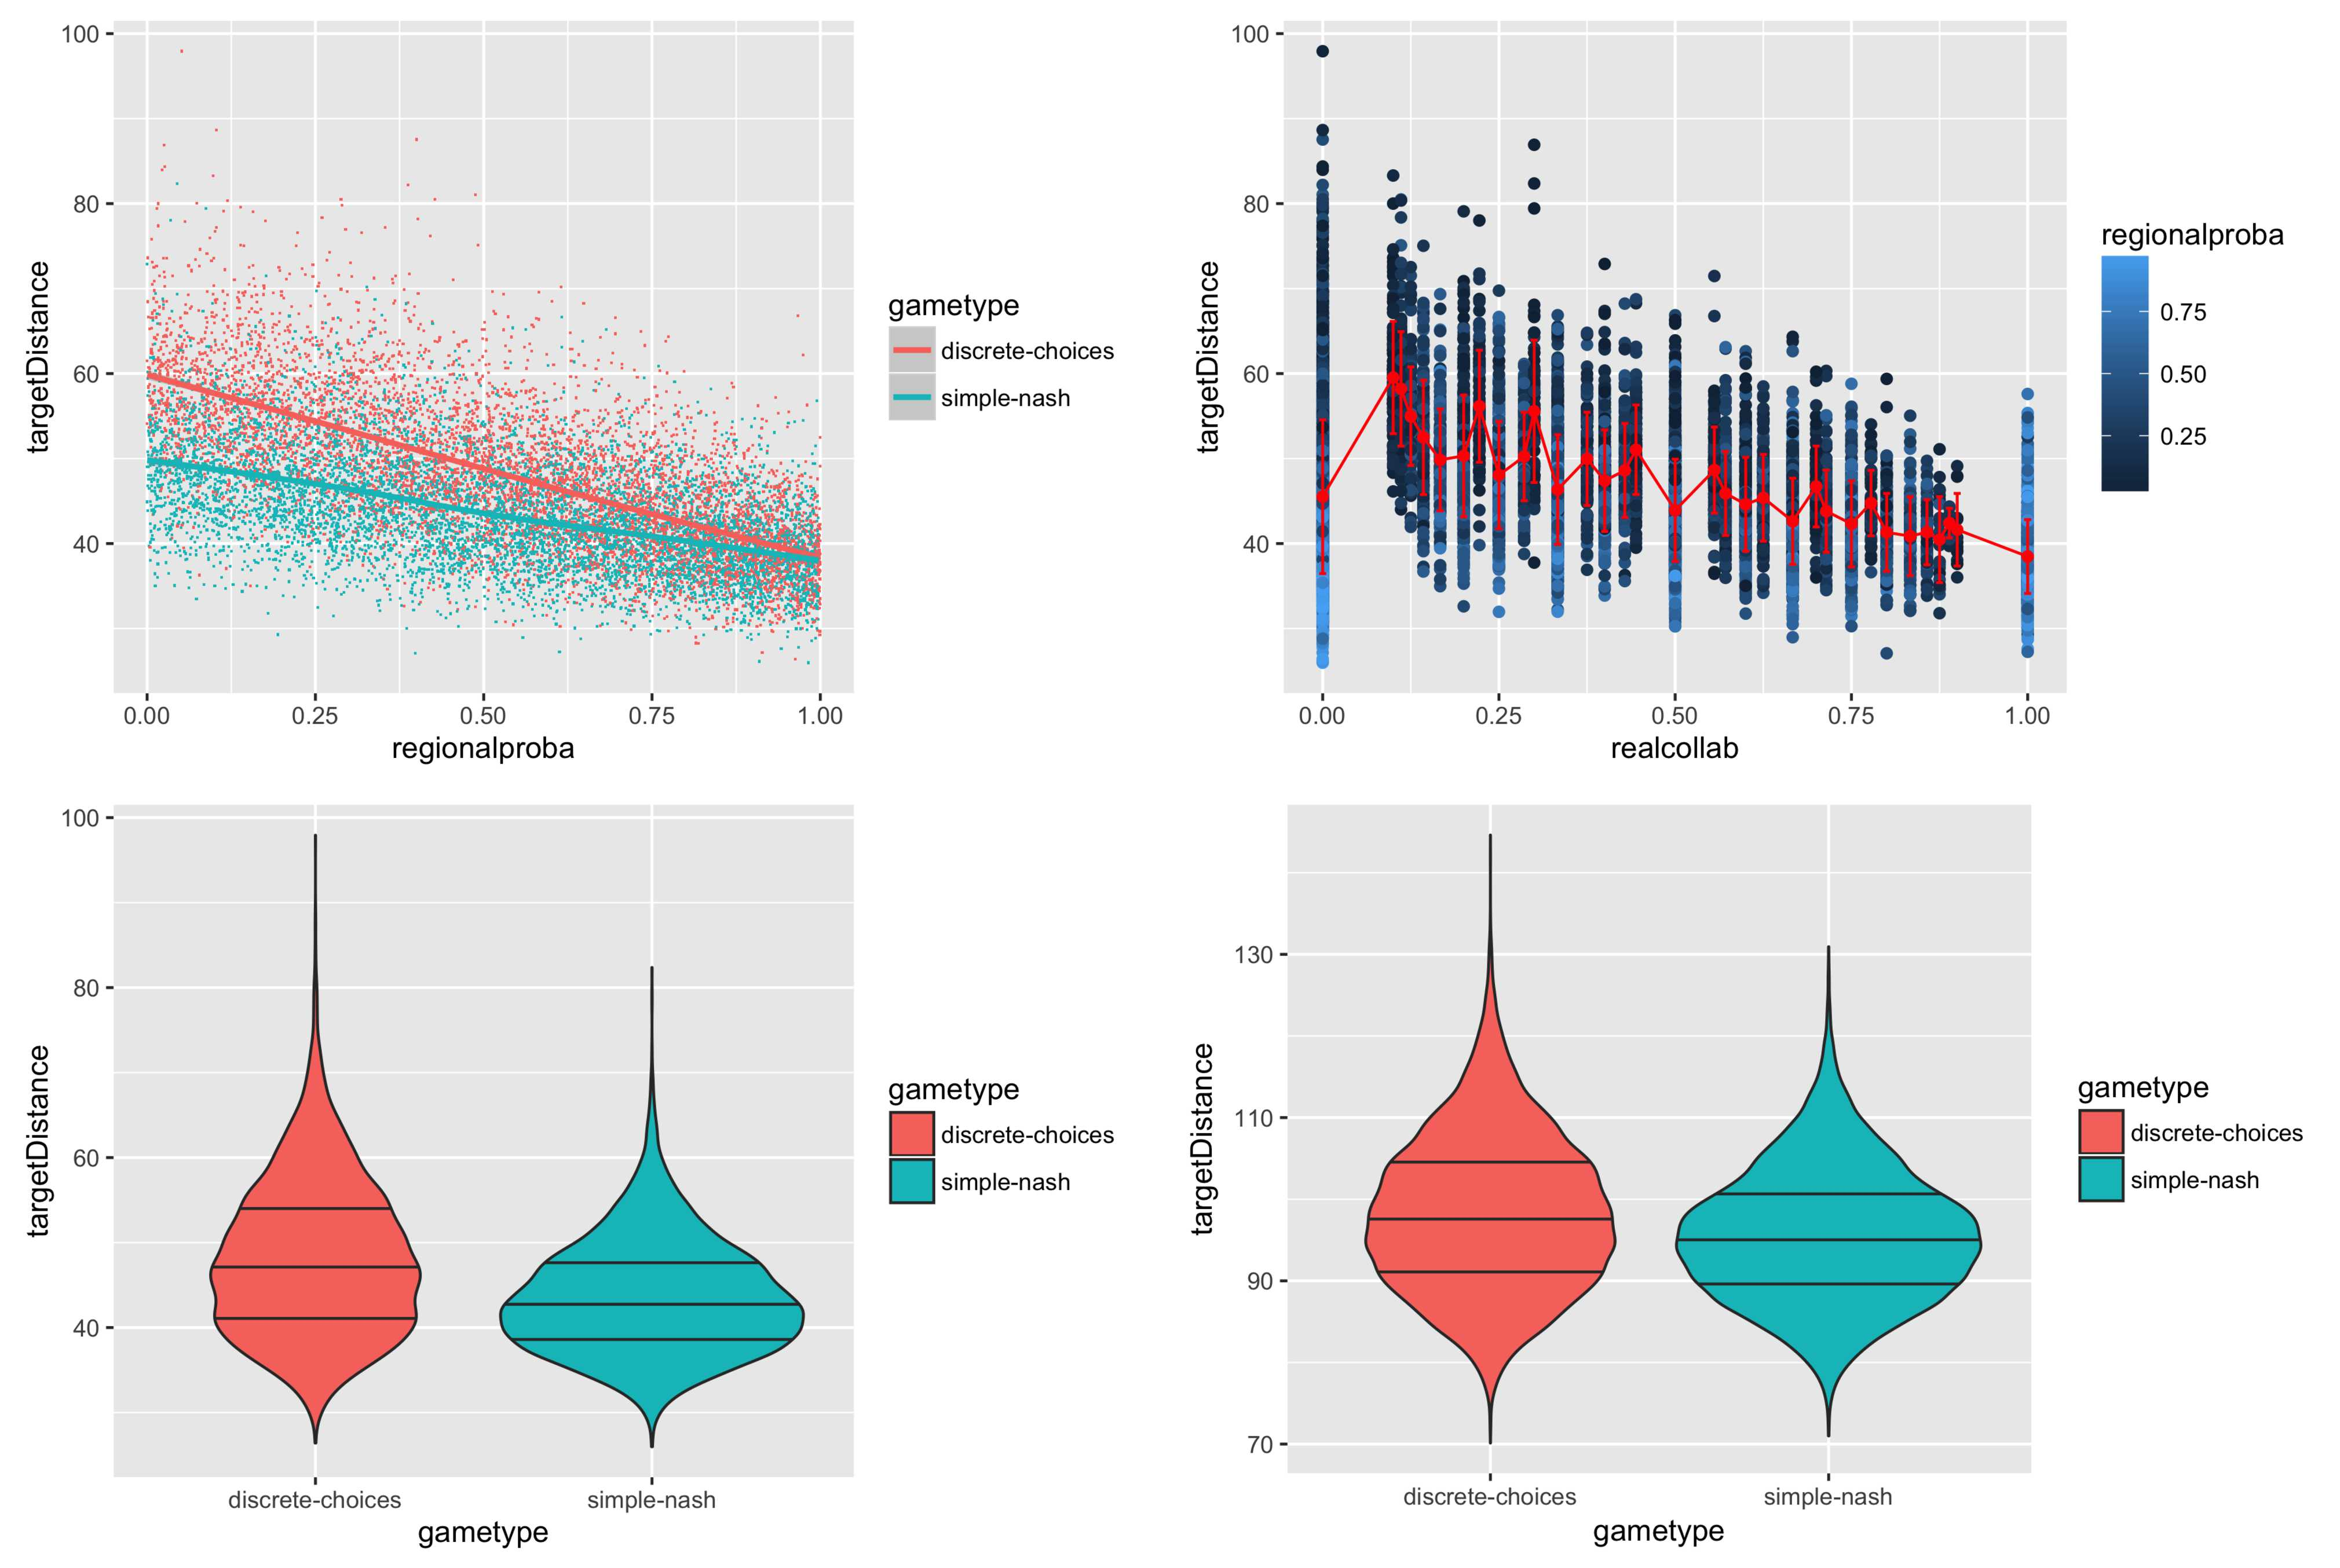
\includegraphics[width=\linewidth]{Figures/Final/7-3-3-fig-lutecia-calib.jpg}
	\caption[Calibration of the Lutecia model][Calibration du modèle Lutecia]{\textbf{Model calibration with fixed land use.}\label{fig:lutecia:calib}}{\textbf{Calibration du modèle à usage du sol fixé.} On prend $\alpha = 0$ pour ne faire évoluer que le réseau, et échantillonnons l'espace des paramètres de gouvernance. (\textit{Haut Gauche}) Distance $d_A$ au réseau cible (targetDistance), dans le cas du réseau réel, en fonction de la probabilité de décision régionale $\xi$ (regionalproba), pour les deux types de jeu (couleur). (\textit{Haut Droite}) Distance $d_A$ en fonction de la probabilité de collaboration observée (realcollab) ; la courbe rouge donne les moyennes avec les barres d'erreur. (\textit{Bas Gauche}) Distribution statistique de la distance en fonction du type de jeu, dans le cas du réseau réel ; (\textit{Bas Droite}) dans le cas du réseau planifié. La différence entre les types de jeux est plus grande dans le cas du réseau réelle en comparaison au réseau planifié.\label{fig:lutecia:calib}}
\end{figure}
%%%%%%%%%%%%%%%



Nous tirons donc de cette expérience les conclusions suivantes, à prendre bien sûr avec prudence :
\begin{itemize}
	\item Une compétition entre les acteurs est plus probable qu'un comportement égoïste dans le cas de décisions locales, puisque le jeu par choix discrets donne de meilleures performances que le Nash pour les faibles valeurs de $\xi$.
	\item Les compromis de collaboration forment des réseaux moins probables que les situations avec pleine collaboration ou avec aucun collaboration.
\end{itemize}


Ces conclusions peuvent être mises en perspective avec la compétition accrue au sein du Delta révélée par~\cite{xu2005city}. Ainsi, cette application du modèle permet d'inférer indirectement des processus de gouvernance.  





\subsubsection{Discussion}{Discussion}

Bien que le modèle ait encore à être exploré plus en profondeur et pour l'ensemble de ses modules, certains développements possibles peuvent retenir notre attention.


\paragraph{Endogenous level of decision}{Niveau de décision endogène}


\bpar{
One interesting aspect to study would be the emergence of larger administrative zones, i.e. the emergence of new levels of governance in polycentric metropolitan areas. The reality is of course not as simple, as bottom-up initiatives such as collaboration between neighbor cities are interlaced with top-down decisions such as e.g. the ``M{\'e}tropole du Grand Paris'' which is a new administrative structure for Paris Area decided at the state level~\cite{gilli2009paris}. It would be however interesting to test conditions for emergence of governance patterns from the bottom-up in a conceptual way by extending the model and adding interactions and fusion between administrative entities.
}{
Une extension pertinente serait l'étude de l'émergence de zones administratives par agrégation, c'est à dire l'émergence de nouveaux niveaux de gouvernance dans une région métropolitaine polycentrique. L'exemple de la Métropole du Grand Paris en est une bonne illustration en la considérant de manière simplifiée, puisqu'elle se situe entre les collectivités locales et la région ainsi que l'état~\cite{gilli2009paris}. Une extension du modèle avec des règles de fusion des entités est une direction potentielle pour étudier cette question.
}


\paragraph{Competition for an external ressource}{Compétition pour une ressource externe}


\bpar{
An interesting extension to the model would be to simulate the competition of territory for an external ressource (an airport for example). The rationale is to explore if different centers of the MCR will tend to cooperate or compete given an externality.
}{
L'influence des territoires extérieurs ou des externalités sur l'évolution d'une MCR est une question ouverte. Dans le cas d'une ressource commune, localisée dans l'emprise de la MCR, des dynamiques de compétition ou de collaboration peuvent s'instituer entre acteurs pour son exploitation. Ce modèle est une solution pour étudier cette situation de manière stylisée, et réaliser ainsi une expérience contrôlée sur les dynamiques de co-évolution, qui permettrait de répondre à des questions plus générales quant au rôle de l'isolation territoriale dans les processus de co-évolution.
}



\stars


Nous avons ainsi posé les premières briques de modèles visant à une intégration plus complexe des processus de co-évolution, en développant le modèle Lutecia qui a ensuite été validé de manière préliminaire et dont les potentialités ont été démontrées par l'application au cas d'étude du Delta de la Rivière des Perles.







\stars




